\documentclass[oneside,openright,a4paper,12pt]{memoir}
\usepackage[utf8]{inputenc}
\usepackage[T1]{fontenc}
\usepackage{amsfonts}
\usepackage{amsthm}
\usepackage{amssymb}
\usepackage{amsmath}
\usepackage{caption}
\usepackage{listings}
\usepackage{algorithm2e}
\usepackage{graphicx}
\usepackage{tikz}

\usepackage[backend=biber,citestyle=authoryear-comp,hyperref=true]{biblatex}
\usepackage[bookmarks,hidelinks]{hyperref}

\pagestyle{ruled}

\theoremstyle{definition}
\newtheorem{df}{Definition}
\newtheorem{thm}{Theorem}

\lstset{
  breaklines=true,
  captionpos=b,
  basicstyle=\ttfamily\footnotesize
}

\addbibresource{common.bib}
\addbibresource{chapters/theory/theory.bib}
\addbibresource{chapters/montecarlo/montecarlo.bib}
\addbibresource{chapters/raytracing/raytracing.bib}

\begin{document}
\title{LIGHT MODELLING ON THE GPU}
\author{Michał Siejak}

\frontmatter
\pagenumbering{gobble}

\begin{titlingpage}
\calccentering{\unitlength}
\begin{adjustwidth*}{\unitlength}{-\unitlength}
\begin{center}
  
\definecolor{cffffff}{RGB}{255,255,255}
\definecolor{c2c2c2b}{RGB}{44,44,43}


\begin{tikzpicture}[scale=0.3,y=0.80pt, x=0.8pt,yscale=-1, inner sep=0pt, outer sep=0pt,
even odd rule]
\begin{scope}[shift={(0,-345.82704)}]
    \path (0.0000,345.8270) -- (425.1970,345.8270) -- (425.1970,841.8900) --
      (0.0000,841.8900) -- (0.0000,345.8270) -- cycle;
    \path[fill=cffffff] (425.1960,841.8900) -- (0.0009,841.8900) --
      (0.0009,345.8270) -- (425.1960,345.8270) -- (425.1960,841.8900) -- cycle;
    \path[fill=c2c2c2b] (208.3210,427.8060) -- (206.5070,427.5820) .. controls
      (204.5570,427.3180) and (201.2100,428.7440) .. (201.0480,428.8120) --
      (199.9860,429.2810) -- (200.9700,429.9300) .. controls (202.8480,431.1660) and
      (204.5860,431.5760) .. (206.0820,431.1220) .. controls (207.9840,430.5450) and
      (208.7660,428.7630) .. (208.8020,428.6900) -- (209.1270,427.9190) --
      (208.3210,427.8060) -- cycle(178.2700,771.0240) -- (178.3300,771.0240) --
      (178.9840,770.2030) -- (178.5240,768.6990) .. controls (178.9810,760.6670) and
      (190.2650,742.3370) .. (190.2650,742.3370) .. controls (190.2650,742.3370) and
      (213.9330,743.0350) .. (217.7220,742.5230) -- (224.3470,766.6090) .. controls
      (221.2050,768.9240) and (220.5990,770.5990) .. (221.1970,771.0190) .. controls
      (226.4800,768.4060) and (236.8900,767.2690) .. (242.6870,768.3620) .. controls
      (243.2460,768.4600) and (254.3510,771.3160) .. (255.3140,770.9110) .. controls
      (254.4160,769.9100) and (252.6780,768.5920) .. (252.4860,767.2490) .. controls
      (252.2830,765.9550) and (252.3450,764.8220) .. (252.3450,764.8220) .. controls
      (250.9900,745.0080) and (260.3750,672.7860) .. (260.3750,671.9030) .. controls
      (261.4530,663.8700) and (263.6350,671.0680) .. (263.6350,671.0680) .. controls
      (263.6350,671.0680) and (282.6420,762.7330) .. (283.8900,768.9820) --
      (283.9340,769.2560) -- (284.4000,770.7110) -- (288.4470,770.7160) --
      (288.9350,768.9820) .. controls (292.9000,754.9790) and (315.9760,674.4510) ..
      (315.9760,674.1680) .. controls (317.8870,668.1570) and (319.8010,673.0450) ..
      (319.8010,673.0450) .. controls (322.8380,676.4970) and (325.0390,765.7940) ..
      (324.9020,765.9700) .. controls (319.8340,768.9140) and (320.7520,771.0190) ..
      (320.8260,771.0190) .. controls (332.0310,765.3500) and (353.3650,770.9160) ..
      (353.6870,770.6720) -- (344.6440,762.2690) -- (344.6440,762.2690) .. controls
      (342.4470,753.8850) and (335.0840,638.3770) .. (335.2240,635.1500) .. controls
      (334.7030,632.7810) and (340.4200,629.2560) .. (340.7670,629.2560) .. controls
      (329.4200,631.3700) and (319.2240,630.3250) .. (314.1750,629.3630) .. controls
      (311.2400,628.6900) and (317.1770,631.7660) .. (316.6460,634.0610) .. controls
      (315.3080,647.5470) and (292.3920,716.9410) .. (292.5840,716.7070) .. controls
      (287.4860,711.9120) and (276.7670,637.5180) .. (276.7280,636.4870) .. controls
      (276.3360,633.1670) and (282.0940,630.5790) .. (281.1290,629.2610) .. controls
      (269.0080,634.7250) and (251.7520,629.2660) .. (251.7520,629.2660) .. controls
      (249.8260,630.1490) and (255.6010,632.4200) .. (255.4370,637.4200) .. controls
      (255.2790,642.4790) and (246.1970,745.2620) .. (244.5950,754.3000) .. controls
      (244.0890,757.2390) and (243.6110,760.4080) .. (242.5450,763.2210) --
      (241.5410,761.7270) .. controls (231.0290,741.8440) and (225.1050,694.7200) ..
      (225.5000,692.8160) .. controls (225.8160,690.9110) and (229.7220,689.7830) ..
      (229.7220,689.7830) -- (205.8310,689.5930) .. controls (205.4770,695.5160) and
      (176.0100,758.0160) .. (169.1710,764.0210) -- (169.1450,763.9970) .. controls
      (169.1450,763.9970) and (169.9210,643.9390) .. (169.9030,637.6880) .. controls
      (169.8200,632.7470) and (176.1290,629.2610) .. (176.1290,629.2610) --
      (175.2160,629.3980) .. controls (171.6760,630.4380) and (167.2470,630.9600) ..
      (162.4040,630.9600) .. controls (157.6080,630.9600) and (153.2380,630.3450) ..
      (149.7160,629.2610) .. controls (148.2190,628.9630) and (147.9310,629.4120) ..
      (147.9310,629.5240) -- (149.6200,631.7220) .. controls (157.9260,639.3340) and
      (148.8150,686.7020) .. (148.2380,687.7380) .. controls (109.4570,801.8490) and
      (94.0138,734.7050) .. (94.0138,734.7050) .. controls (89.8341,716.1260) and
      (99.5530,640.4520) .. (99.8342,640.2910) .. controls (102.4340,635.1350) and
      (110.4900,630.2820) .. (110.3070,629.6810) -- (110.0820,629.4320) .. controls
      (94.9875,636.4190) and (71.1739,629.1440) .. (70.9962,629.2760) --
      (70.9378,629.2900) -- (70.9378,629.4420) .. controls (69.9514,629.9740) and
      (79.6311,634.3390) .. (79.9514,638.2940) .. controls (79.8976,640.2470) and
      (74.5041,726.1460) .. (74.5041,725.8230) .. controls (73.2180,770.4720) and
      (99.5042,771.0190) .. (99.5042,771.0190) .. controls (134.3140,770.4470) and
      (149.8090,704.7110) .. (150.1180,703.0300) .. controls (150.4970,701.3120) and
      (152.3690,702.0440) .. (152.3690,702.0440) -- (152.7240,762.9570) --
      (151.5030,766.2090) -- (148.7070,771.0190) .. controls (157.7650,767.9860) and
      (166.9540,768.6260) .. (176.1050,770.5940) .. controls (177.2340,770.8460) and
      (178.0030,770.9940) .. (178.2700,771.0240) -- cycle(337.2460,547.3130) --
      (337.2460,547.3130) .. controls (331.9100,547.6110) and (318.1540,544.5790) ..
      (305.9270,509.8960) .. controls (305.2790,508.0940) and (304.3120,507.1660) ..
      (303.2910,507.3470) .. controls (301.9780,507.5770) and (301.2550,509.4570) ..
      (301.2550,512.6450) -- (301.2550,512.7180) .. controls (301.2590,523.5530) and
      (302.6230,559.9940) .. (319.8690,574.1830) .. controls (325.7580,579.0370) and
      (332.9980,580.7020) .. (341.3140,579.2710) .. controls (338.6480,588.6700) and
      (333.4530,594.6120) .. (327.3400,595.2180) .. controls (318.9940,596.0240) and
      (309.8980,587.1960) .. (301.7630,570.3450) .. controls (299.7950,566.1170) and
      (297.1340,557.8550) .. (294.3220,549.1100) .. controls (288.2870,530.5020) and
      (284.1090,518.2110) .. (280.8880,516.9420) .. controls (279.6330,516.4540) and
      (278.7790,516.7960) .. (278.2970,517.1860) .. controls (276.9000,518.2990) and
      (275.3450,521.7320) .. (277.7520,538.6360) .. controls (279.7810,550.2330) and
      (284.0920,556.9810) .. (287.8420,559.8320) .. controls (282.8260,560.8780) and
      (274.2380,560.6620) .. (263.4700,526.3610) .. controls (262.2770,522.6740) and
      (260.9590,520.8680) .. (259.4860,520.9800) .. controls (257.6500,521.1360) and
      (256.8530,524.1490) .. (256.4900,526.6340) .. controls (255.7280,531.7030) and
      (258.3280,541.7120) .. (260.4430,546.6640) .. controls (253.1970,540.4770) and
      (240.4160,523.7630) .. (245.1190,509.3100) .. controls (248.0840,514.5590) and
      (249.8850,516.4340) .. (249.9490,516.5120) -- (250.3200,516.8930) --
      (250.7690,516.5710) -- (257.1810,511.7520) -- (266.2400,516.6100) --
      (266.8340,516.9420) -- (267.1070,516.3070) -- (270.1130,509.3100) --
      (279.1890,512.8500) -- (279.7650,513.0940) -- (279.9860,512.4600) --
      (281.9510,506.4680) -- (289.8300,510.4870) -- (290.5720,510.8630) --
      (290.7220,510.0720) -- (292.7440,501.0630) -- (302.3920,505.2430) --
      (303.2620,505.6280) -- (303.2620,504.6670) -- (303.2580,493.7730) --
      (312.7990,493.7680) -- (313.4230,493.7680) -- (313.4230,493.1240) --
      (313.4180,486.6730) -- (321.1770,485.8240) -- (321.7540,485.7600) --
      (321.7240,485.1840) -- (321.3830,469.6420) .. controls (321.3670,469.3400) and
      (321.1190,467.1520) .. (319.7650,466.3510) .. controls (319.3360,466.0970) and
      (318.6480,465.8680) .. (317.6710,466.2540) .. controls (316.0310,466.9520) and
      (314.2240,468.3340) .. (314.0520,470.1450) .. controls (313.9020,471.4150) and
      (314.6930,472.5870) .. (316.1420,473.6850) -- (316.1420,479.9690) .. controls
      (315.9430,480.2770) and (314.5170,481.9860) .. (308.6030,480.0770) --
      (307.7790,479.8030) -- (307.7790,480.6680) .. controls (307.7790,487.4550) and
      (306.5040,488.2210) .. (300.0000,489.0810) -- (299.5990,489.1340) --
      (299.4680,489.5100) .. controls (298.5060,492.4600) and (297.7110,494.5930) ..
      (296.1420,495.2230) .. controls (294.7520,495.7940) and (292.5640,495.2380) ..
      (289.2850,493.4850) -- (288.5150,493.0850) -- (288.3650,493.9240) .. controls
      (288.2400,494.6670) and (288.1210,495.3550) .. (288.0170,496.0340) .. controls
      (287.6520,498.5290) and (287.3510,500.5060) .. (286.2050,501.0440) .. controls
      (285.1720,501.5660) and (283.2130,500.9800) .. (280.2340,499.2860) --
      (279.5660,498.9000) -- (279.3120,499.6520) .. controls (279.1400,500.2040) and
      (278.9840,500.7750) .. (278.8080,501.3220) .. controls (278.0620,503.9150) and
      (277.3280,506.3510) .. (276.0250,506.6930) .. controls (274.9200,506.9810) and
      (273.1340,505.9220) .. (270.7620,503.5730) -- (270.2280,503.0600) --
      (269.7890,503.6510) .. controls (266.9660,507.6450) and (264.4000,509.5840) ..
      (262.2010,509.4470) .. controls (260.5430,509.3440) and (258.9980,508.0360) ..
      (257.6330,505.5210) -- (257.2400,504.7790) -- (256.6360,505.3700) .. controls
      (254.1560,507.8550) and (252.4340,508.8710) .. (251.0270,508.6950) .. controls
      (249.7480,508.5240) and (248.5210,507.3670) .. (247.0920,504.9350) --
      (247.0430,504.8620) -- (246.9980,504.8030) .. controls (246.3510,504.1880) and
      (245.4570,503.6210) .. (244.6410,503.1530) .. controls (244.3710,502.9970) and
      (244.0740,502.8060) .. (243.8300,502.6500) .. controls (244.2540,502.6060) and
      (244.9450,502.5620) .. (246.0920,502.5620) -- (246.3260,502.5570) .. controls
      (253.5270,502.5520) and (272.6400,502.5470) .. (286.0920,493.4800) .. controls
      (300.7870,483.6170) and (315.9040,472.1670) .. (309.9470,461.1120) .. controls
      (309.9800,459.5150) and (310.6600,458.7630) .. (312.2850,457.1130) .. controls
      (313.4720,455.9120) and (314.0330,452.9530) .. (314.0330,450.7410) .. controls
      (314.0330,449.4230) and (313.8630,447.6890) .. (313.0170,446.8440) --
      (312.5540,446.3850) -- (312.1350,446.8440) .. controls (311.2400,447.7280) and
      (310.7970,448.7190) .. (310.3960,449.6860) .. controls (309.7130,451.2490) and
      (308.9800,452.7380) .. (306.3240,453.9980) .. controls (305.5040,452.3470) and
      (304.8790,450.9560) .. (304.4100,449.8330) .. controls (303.1010,446.8930) and
      (302.4510,445.3890) .. (300.3960,445.3890) -- (299.7460,445.3990) --
      (299.7460,446.0440) .. controls (299.7460,446.9810) and (300.0880,448.0940) ..
      (300.4450,449.2860) .. controls (300.9470,451.0780) and (301.5290,453.1090) ..
      (300.9180,454.6520) .. controls (297.9490,455.8090) and (294.5660,460.0570) ..
      (294.5660,462.8210) -- (294.5660,463.6560) -- (295.3670,463.4360) .. controls
      (296.3470,463.1430) and (297.1840,462.7870) .. (297.8670,462.4990) .. controls
      (298.4040,462.2790) and (299.1270,461.9520) .. (299.3220,462.0200) .. controls
      (299.3550,462.0300) and (299.5120,462.2200) .. (299.5120,463.2900) .. controls
      (299.5120,464.0030) and (299.4530,464.6760) .. (299.4140,465.3210) .. controls
      (299.2440,467.6350) and (299.1210,469.6320) .. (301.4160,471.9320) --
      (302.1930,472.7040) -- (302.4570,471.6490) .. controls (303.8630,466.3410) and
      (306.2790,463.6800) .. (306.8840,463.6900) .. controls (306.9240,463.7240) and
      (307.0370,463.8950) .. (307.0370,464.6180) .. controls (307.0370,468.4800) and
      (306.0050,473.6800) .. (297.8900,479.6370) .. controls (292.3630,483.6750) and
      (278.1050,493.3580) .. (264.7610,495.6140) .. controls (264.7770,495.6140) and
      (262.1270,496.0630) .. (262.1270,496.0630) .. controls (252.4720,497.7570) and
      (246.5150,498.7000) .. (242.3550,492.6550) .. controls (249.4310,492.2490) and
      (287.1950,489.4130) .. (297.4510,474.7990) -- (297.7110,474.4180) --
      (297.4370,474.0560) .. controls (294.9860,470.8580) and (289.2670,460.7600) ..
      (292.0080,452.4400) .. controls (293.5930,447.6650) and (297.7690,444.3050) ..
      (304.4200,442.4350) .. controls (310.7710,440.9560) and (315.9430,443.6850) ..
      (319.1400,446.2390) .. controls (325.0970,450.9900) and (329.2540,458.9780) ..
      (329.2570,465.7070) .. controls (329.3900,472.1620) and (330.4680,493.5920) ..
      (339.3550,498.6220) .. controls (342.0760,500.1650) and (345.3510,499.9450) ..
      (348.9650,498.1480) .. controls (348.3060,501.4490) and (346.1680,506.0630) ..
      (342.0170,507.3620) .. controls (337.6720,508.7340) and (332.2460,505.8290) ..
      (326.3730,498.9540) .. controls (325.7030,498.2750) and (324.7460,497.4990) ..
      (323.7790,497.8890) .. controls (322.8220,498.2800) and (322.3920,499.7450) ..
      (322.3920,502.7230) .. controls (322.3920,502.9970) and (322.9450,529.6520) ..
      (334.9570,538.2600) .. controls (338.5890,540.8630) and (342.8810,541.4100) ..
      (347.7140,540.0620) .. controls (346.4060,543.5530) and (342.4860,547.0050) ..
      (337.2460,547.3130) -- cycle(291.9980,559.3830) -- (291.9980,559.3830) ..
      controls (292.0110,559.4130) and (291.7050,558.9100) .. (291.7050,558.9100) ..
      controls (291.6850,558.8850) and (290.9270,557.7960) .. (290.9270,557.7960) ..
      controls (290.9630,557.8310) and (290.5920,557.2590) .. (290.5920,557.2590) ..
      controls (290.5920,557.2350) and (289.9660,556.2830) .. (289.9660,556.2830) --
      (289.6070,555.7210) .. controls (289.6170,555.7310) and (289.0970,554.8960) ..
      (289.0970,554.8960) .. controls (289.0970,554.9450) and (288.8060,554.3780) ..
      (288.8060,554.3780) .. controls (288.7950,554.3340) and (288.2910,553.5440) ..
      (288.2910,553.5440) -- (287.9880,553.0450) .. controls (288.0230,553.0550) and
      (287.5640,552.2980) .. (287.5640,552.2980) .. controls (287.5780,552.3130) and
      (287.3200,551.8100) .. (287.3200,551.8100) .. controls (287.3340,551.8340) and
      (286.9710,551.1320) .. (286.9710,551.1320) .. controls (287.0020,551.1610) and
      (286.7730,550.6580) .. (286.7730,550.6580) .. controls (286.7260,550.6140) and
      (286.3900,549.9790) .. (286.3900,549.9790) .. controls (286.4230,550.0230) and
      (286.2360,549.5690) .. (286.2360,549.5690) -- (285.9370,548.9340) .. controls
      (285.9370,548.9630) and (285.7670,548.5430) .. (285.7670,548.5430) .. controls
      (285.7580,548.5090) and (285.5450,548.0260) .. (285.5130,547.9770) --
      (285.4080,547.6300) -- (285.4080,547.5960) -- (285.3880,547.5470) --
      (285.1620,547.0640) -- (285.0930,546.8200) -- (285.0930,546.7610) --
      (285.0820,546.7170) -- (284.8920,546.1700) .. controls (284.8920,546.1700) and
      (284.8380,545.9990) .. (284.8240,545.9410) -- (284.6830,545.4230) --
      (284.6830,545.3840) -- (284.6750,545.3650) -- (284.5640,545.1210) --
      (284.4820,544.6960) .. controls (284.4820,544.7110) and (284.4300,544.5050) ..
      (284.4300,544.4470) -- (284.3840,544.0760) -- (284.3840,544.0220) --
      (284.3690,543.9680) -- (284.3240,543.7540) .. controls (284.3240,543.7830) and
      (284.2340,543.4210) .. (284.2340,543.3730) -- (284.2340,543.2160) .. controls
      (284.2340,543.2360) and (284.2050,542.8600) .. (284.2050,542.8600) .. controls
      (284.2050,542.8940) and (284.2030,542.6990) .. (284.2030,542.6990) --
      (284.2030,542.3620) -- (284.2030,542.2150) .. controls (284.2030,542.2590) and
      (284.2340,541.8880) .. (284.2340,541.8880) .. controls (284.2340,541.9030) and
      (284.2340,541.8740) .. (284.2320,541.8540) -- (284.3510,541.5710) .. controls
      (284.3510,541.5270) and (284.3690,541.4530) .. (284.3690,541.4530) .. controls
      (284.3810,541.4190) and (284.3940,541.3070) .. (284.4280,541.2090) --
      (284.4280,541.1510) -- (284.5270,540.8870) -- (284.6720,540.6720) --
      (284.7400,540.5310) .. controls (284.7830,540.4960) and (284.7830,540.4380) ..
      (284.8320,540.4040) -- (284.8320,540.3790) -- (284.9000,540.3160) --
      (284.9300,540.2620) -- (284.9960,540.2180) -- (285.0450,540.1790) --
      (285.1910,540.0670) -- (285.3160,539.9790) -- (285.3160,539.9640) .. controls
      (285.3550,539.9640) and (285.4530,539.9060) .. (285.4530,539.9060) --
      (285.5500,539.8670) .. controls (285.5760,539.8570) and (285.6150,539.8470) ..
      (285.6150,539.8470) -- (285.6130,539.8570) .. controls (286.6750,540.8730) and
      (290.0860,550.8680) .. (293.0620,560.8430) -- (291.9980,559.3830) --
      cycle(257.7970,579.7300) -- (257.7970,579.7300) -- (258.2260,580.1600) --
      (258.6540,579.7300) -- (259.0310,579.3440) .. controls (263.2540,575.1600) and
      (268.4800,569.9600) .. (272.9180,570.9410) .. controls (275.2630,571.4630) and
      (277.2650,573.8070) .. (278.8510,577.7670) .. controls (275.0370,577.9230) and
      (267.7500,578.9540) .. (267.7540,582.6990) .. controls (267.7540,583.6260) and
      (268.0150,584.3200) .. (268.5250,584.7980) .. controls (269.5250,585.6920) and
      (271.1480,585.5260) .. (272.8610,585.3160) .. controls (273.5510,585.2480) and
      (274.2550,585.1650) .. (274.9120,585.1650) .. controls (277.7690,585.1650) and
      (286.4140,585.1600) .. (286.4160,591.7320) .. controls (286.4200,598.2400) and
      (283.4470,599.6420) .. (281.5860,599.9060) .. controls (281.7710,598.0990) and
      (281.4140,595.7700) .. (279.6870,593.7970) .. controls (277.9860,591.8150) and
      (274.3460,589.5880) .. (266.6830,590.2330) -- (265.7500,590.3010) --
      (266.1760,591.1310) .. controls (266.4350,591.6640) and (266.8000,592.3130) ..
      (267.2110,593.0890) .. controls (267.3960,593.4460) and (267.6350,593.8750) ..
      (267.8690,594.2710) -- (267.7600,594.3000) -- (267.8960,594.3590) .. controls
      (270.4180,599.0850) and (274.3630,607.0880) .. (271.9240,610.9110) .. controls
      (270.8400,612.5470) and (268.5540,613.2650) .. (265.1950,613.1570) .. controls
      (267.2620,606.0090) and (264.4220,601.1600) .. (261.5680,598.3430) .. controls
      (258.6440,595.4330) and (254.8550,592.1570) .. (251.2730,592.4550) .. controls
      (249.6720,592.6060) and (248.3180,593.4650) .. (247.2110,595.0280) .. controls
      (246.2360,596.6290) and (246.2580,598.2060) .. (247.2110,599.5200) .. controls
      (248.3160,601.0530) and (250.5410,601.9460) .. (252.8340,601.9320) .. controls
      (251.5290,603.3770) and (249.9760,604.4460) .. (248.1970,604.6520) .. controls
      (245.6750,604.9150) and (243.1110,603.8020) .. (240.7190,601.4190) .. controls
      (239.1540,599.8710) and (238.6340,597.3080) .. (239.3140,594.7350) .. controls
      (240.5640,590.1650) and (245.2010,586.5360) .. (252.0640,584.8030) --
      (252.5350,584.6760) -- (252.5350,584.1780) .. controls (252.5310,578.4220) and
      (250.2320,573.6950) .. (244.8790,568.4020) -- (244.4490,567.9430) --
      (244.0020,568.3920) -- (243.7180,568.6700) .. controls (242.7520,569.6420) and
      (241.7440,570.6430) .. (240.5680,570.4040) .. controls (238.5130,569.9940) and
      (235.9800,566.1700) .. (233.0350,559.0320) -- (233.0060,558.9100) --
      (232.9270,558.8510) .. controls (232.0170,557.1860) and (237.0450,539.6520) ..
      (237.9860,538.3920) -- (238.1130,538.2750) .. controls (238.1010,538.2890) and
      (238.1380,538.1280) .. (238.1380,538.1280) .. controls (238.3940,537.1420) and
      (239.1170,535.6670) .. (239.7990,535.6090) .. controls (240.0170,535.5940) and
      (240.8160,535.7120) .. (242.0490,538.2310) .. controls (242.5640,539.2860) and
      (243.1270,540.3600) .. (243.7150,541.5070) .. controls (246.8100,547.4160) and
      (250.3040,554.1250) .. (249.2600,560.7550) .. controls (247.8790,567.6300) and
      (256.9080,578.8850) .. (257.7910,579.7300) -- (257.7970,579.7300) --
      cycle(272.9060,595.5450) -- (272.9060,595.5450) .. controls
      (273.7750,595.7700) and (274.5020,596.1650) .. (275.0840,596.7460) .. controls
      (276.0040,597.6450) and (276.4290,598.8410) .. (276.6600,599.9200) .. controls
      (275.7810,598.1770) and (274.5510,596.7070) .. (272.9060,595.5450) --
      cycle(230.9300,525.1600) -- (230.9300,525.1600) -- (230.1540,524.6660) --
      (229.9720,525.5600) .. controls (229.3570,528.3580) and (227.4550,535.5460) ..
      (225.5990,538.2650) .. controls (224.7570,536.8490) and (223.8880,535.2130) ..
      (223.0450,533.5780) .. controls (221.4310,530.4230) and (219.8960,527.4450) ..
      (218.3730,525.9510) -- (217.6030,525.1940) -- (217.3300,526.2190) .. controls
      (216.4180,529.4470) and (215.8920,531.9220) .. (215.4820,533.9100) .. controls
      (214.9260,536.4930) and (214.5720,538.0600) .. (213.8390,539.1200) .. controls
      (209.8890,534.8720) and (206.9200,527.3470) .. (206.8730,527.2740) --
      (206.2070,525.5210) -- (205.7010,527.3380) -- (202.7060,537.9870) .. controls
      (201.3860,536.9320) and (198.4140,534.0170) .. (198.2430,528.9050) --
      (198.1750,526.5370) -- (197.0600,528.6410) -- (193.1360,536.1360) .. controls
      (191.5620,534.1880) and (187.1350,527.1130) .. (189.6040,512.7330) .. controls
      (192.6720,518.0750) and (196.7100,522.2400) .. (196.8950,522.4250) --
      (197.7240,523.2410) -- (197.9580,522.1030) -- (199.7320,513.5480) .. controls
      (201.9010,516.7560) and (204.5960,521.1750) .. (204.5960,522.4500) --
      (204.5960,523.9640) -- (205.6890,522.8940) .. controls (208.5670,519.9940) and
      (211.2630,515.7410) .. (212.0340,513.1920) .. controls (214.0580,515.3310) and
      (216.7440,519.1200) .. (217.2970,522.8890) -- (218.5560,522.7770) --
      (218.4880,523.0360) .. controls (218.5470,522.9380) and (218.8550,522.4110) ..
      (219.1950,521.8490) .. controls (221.6350,517.8600) and (223.9390,513.9780) ..
      (224.9180,511.5810) .. controls (227.0960,516.7760) and (228.8830,523.2210) ..
      (228.9020,523.2990) -- (229.1090,524.0900) -- (229.8180,523.6700) .. controls
      (230.0550,523.5090) and (234.9470,520.5110) .. (237.9260,515.1840) .. controls
      (237.7710,524.8520) and (236.6290,527.8890) .. (233.2750,531.4590) .. controls
      (232.9120,526.7270) and (231.0120,525.2140) .. (230.9300,525.1600) --
      cycle(227.5170,549.9350) -- (227.5170,549.9350) -- (225.6970,548.2060) --
      (225.2600,547.7770) -- (224.8120,548.2120) .. controls (224.7150,548.3140) and
      (222.6830,550.5700) .. (220.3650,558.9440) .. controls (217.9470,555.9070) and
      (214.3770,548.2550) .. (214.3280,548.1680) -- (213.9820,547.4300) .. controls
      (214.1370,547.1720) and (214.2950,546.8540) .. (214.2950,546.8540) --
      (219.1770,538.0550) .. controls (220.7460,541.7120) and (222.3650,546.0290) ..
      (222.3750,546.0870) -- (222.7790,547.1220) -- (223.4630,546.2490) .. controls
      (225.4840,543.7040) and (228.5760,540.3890) .. (230.2560,539.5400) .. controls
      (230.0600,545.1600) and (228.2770,548.7290) .. (227.5170,549.9350) --
      cycle(221.4880,566.7660) -- (221.4880,566.7660) .. controls
      (220.4470,567.7670) and (218.9590,567.1230) .. (218.8790,567.0930) --
      (218.0130,566.7080) .. controls (218.0040,566.7080) and (218.0040,567.6790) ..
      (218.0040,567.6790) .. controls (218.0040,567.7040) and (217.9250,570.8430) ..
      (215.8460,574.6520) .. controls (213.8750,573.8800) and (213.0400,572.2200) ..
      (211.8930,569.7450) .. controls (211.6080,569.1200) and (211.3140,568.4750) ..
      (210.9550,567.7770) -- (210.2210,566.3170) -- (209.7960,567.8790) .. controls
      (208.5330,572.4110) and (211.1940,577.4250) .. (216.1840,579.8080) .. controls
      (216.9490,580.1840) and (217.3100,580.6770) .. (217.2830,581.3270) .. controls
      (217.2220,582.9620) and (214.8220,585.2570) .. (212.8890,586.0580) .. controls
      (212.1660,586.3460) and (211.7070,586.3460) .. (211.5390,586.2290) .. controls
      (197.2180,552.3280) and (197.5720,545.1990) .. (198.5560,541.0440) .. controls
      (201.8470,542.7530) and (204.4540,546.8150) .. (204.4930,546.8640) --
      (205.2650,548.1480) -- (205.6310,546.6930) .. controls (205.6410,546.6390) and
      (206.5830,542.9240) .. (207.9770,539.4560) .. controls (209.8450,541.6490) and
      (213.1820,546.8100) .. (213.2380,546.8780) -- (213.5580,547.3570) --
      (213.1900,548.1630) -- (209.3030,556.9270) .. controls (208.2480,555.9160) and
      (206.0170,553.6170) .. (203.7900,550.3110) -- (202.6520,550.7990) .. controls
      (204.4710,559.2610) and (206.8680,562.0540) .. (209.5960,564.6030) --
      (210.6550,565.5890) -- (210.6550,564.1590) .. controls (210.6870,563.4800) and
      (212.7500,558.8660) .. (214.3590,556.6100) .. controls (215.1890,559.7840) and
      (218.4040,563.2070) .. (218.8420,563.6220) .. controls (219.3240,564.1240) and
      (219.8670,564.5590) .. (220.3360,564.9400) .. controls (220.9740,565.4720) and
      (221.6910,566.0730) .. (221.7160,566.4050) .. controls (221.7160,566.5420) and
      (221.5760,566.6980) .. (221.4880,566.7660) -- cycle(220.4450,596.9560) --
      (220.4450,596.9560) .. controls (220.8940,598.2450) and (220.8240,599.3390) ..
      (220.1640,600.2960) .. controls (218.3710,602.8840) and (213.0110,603.7580) ..
      (211.7100,603.7580) .. controls (210.3890,603.7580) and (201.1680,602.6060) ..
      (201.1650,597.9380) .. controls (201.1650,594.0560) and (208.8070,592.8700) ..
      (211.7410,592.7570) .. controls (216.3450,592.7470) and (220.1150,596.6240) ..
      (220.4450,596.9560) -- cycle(225.5290,630.2670) -- (225.5290,630.2670) ..
      controls (229.3090,633.5580) and (234.1030,634.9690) .. (239.7710,634.5730) ..
      controls (238.2930,637.3470) and (235.4740,639.1290) .. (232.0780,639.2510) ..
      controls (226.4960,639.4120) and (221.3240,635.4770) .. (218.2600,628.7090) --
      (217.3650,626.7710) -- (217.0660,628.8650) .. controls (216.2560,634.3000) and
      (223.8650,646.7270) .. (236.0230,653.3180) .. controls (234.8360,654.5200) and
      (233.1010,655.3550) .. (230.9410,655.4130) .. controls (226.6250,655.5650) and
      (221.9450,653.2310) .. (218.4100,649.1540) -- (217.7890,648.4310) --
      (217.3810,649.3000) .. controls (216.6780,650.7700) and (217.5990,652.4690) ..
      (218.5920,654.2750) .. controls (219.3690,655.6770) and (220.1480,657.1270) ..
      (220.1480,658.4500) .. controls (220.1480,659.3730) and (219.9450,667.4540) ..
      (212.9420,671.8830) .. controls (205.9340,667.4590) and (205.6890,659.3830) ..
      (205.6890,658.4550) .. controls (205.6890,657.1220) and (206.4630,655.6820) ..
      (207.2370,654.2810) .. controls (208.2110,652.4690) and (209.1190,650.7750) ..
      (208.4290,649.3050) -- (208.0250,648.4310) -- (207.4040,649.1580) .. controls
      (203.8930,653.2110) and (199.2490,655.5550) .. (194.9470,655.4480) .. controls
      (192.7740,655.3740) and (191.0290,654.5640) .. (189.8250,653.3380) .. controls
      (201.9050,646.7510) and (209.5440,634.3440) .. (208.7970,628.9140) --
      (208.4920,626.7610) -- (207.5840,628.7190) .. controls (204.5150,635.4870) and
      (199.3250,639.4370) .. (193.7610,639.2660) .. controls (190.3670,639.1340) and
      (187.5970,637.3760) .. (186.1390,634.6420) .. controls (191.6400,635.2810) and
      (196.3570,634.0750) .. (200.0770,630.9450) .. controls (208.1900,624.1580) and
      (209.2200,611.0190) .. (209.3390,608.2260) -- (216.5000,608.2210) .. controls
      (216.6330,610.9550) and (217.6810,623.3770) .. (225.5290,630.2670) --
      cycle(193.7980,558.8560) -- (193.7980,558.8560) -- (193.7300,558.9150) --
      (193.6780,559.0320) .. controls (190.7430,566.1700) and (188.2310,569.9990) ..
      (186.1760,570.4090) .. controls (184.9670,570.6380) and (183.9790,569.6420) ..
      (183.0040,568.6800) -- (182.7450,568.4110) -- (182.2910,567.9530) --
      (181.8450,568.4110) .. controls (176.4950,573.7140) and (174.2150,578.4410) ..
      (174.2180,584.1980) -- (174.2180,584.6910) -- (174.7080,584.8180) .. controls
      (181.5340,586.5360) and (186.1760,590.1650) .. (187.4180,594.7300) .. controls
      (188.1210,597.3230) and (187.5890,599.8760) .. (186.0390,601.4240) .. controls
      (183.6610,603.8170) and (181.0800,604.9200) .. (178.5560,604.6470) .. controls
      (176.7830,604.4660) and (175.2380,603.4010) .. (173.9350,601.9460) .. controls
      (176.2200,601.9610) and (178.4370,601.0630) .. (179.5570,599.5290) .. controls
      (180.5070,598.2260) and (180.5140,596.6340) .. (179.5910,595.0670) .. controls
      (178.4510,593.4700) and (177.1010,592.6160) .. (175.4940,592.4640) .. controls
      (171.8640,592.1570) and (167.8670,595.6820) .. (165.1770,598.3580) .. controls
      (162.3330,601.1850) and (159.4980,606.0380) .. (161.5540,613.1770) .. controls
      (158.1850,613.2990) and (155.9120,612.5720) .. (154.8400,610.9210) .. controls
      (152.1430,606.7410) and (157.1640,597.4490) .. (159.5650,593.0260) .. controls
      (159.9750,592.2890) and (160.2990,591.6640) .. (160.5580,591.1510) --
      (160.9730,590.3310) -- (160.0450,590.2620) .. controls (152.4160,589.6270) and
      (148.7730,591.8540) .. (147.0740,593.8310) .. controls (145.3630,595.7990) and
      (144.9720,598.1380) .. (145.1720,599.9490) .. controls (143.3140,599.6910) and
      (140.3260,598.2890) .. (140.3230,591.7810) .. controls (140.3210,585.2040) and
      (148.9810,585.2040) .. (151.8080,585.1990) .. controls (152.4620,585.1990) and
      (153.1970,585.2860) .. (153.8910,585.3500) .. controls (155.6020,585.5500) and
      (157.2130,585.7110) .. (158.1940,584.8280) .. controls (158.7120,584.3540) and
      (158.9880,583.6610) .. (158.9880,582.7330) .. controls (158.9860,578.9830) and
      (151.6860,577.9570) .. (147.9020,577.8060) .. controls (149.4840,573.8410) and
      (151.4450,571.5120) .. (153.7730,570.9800) .. controls (158.1800,569.9840) and
      (163.4290,575.1700) .. (167.6330,579.3150) -- (168.0820,579.7540) --
      (168.5050,580.1840) -- (168.9590,579.7540) .. controls (169.9550,578.7630) and
      (178.8130,567.5330) .. (177.4700,560.7600) .. controls (176.4270,554.1540) and
      (179.9110,547.4450) .. (182.9870,541.5220) .. controls (183.6050,540.3790) and
      (184.1520,539.3000) .. (184.6740,538.2600) .. controls (185.9020,535.7260) and
      (186.7000,535.6140) .. (186.9280,535.6280) .. controls (187.5970,535.6870) and
      (188.2970,537.1610) .. (188.5780,538.1330) -- (188.6140,538.2990) --
      (188.7510,538.4260) .. controls (189.6790,539.6520) and (194.7080,557.1370) ..
      (193.7980,558.8560) -- cycle(149.3660,600.3010) -- (149.3660,600.3010) ..
      controls (149.5760,599.1440) and (150.0280,597.7860) .. (151.0000,596.8000) ..
      controls (151.6030,596.1800) and (152.4160,595.7990) .. (153.3070,595.5740) ..
      controls (151.5540,596.8190) and (150.2530,598.4070) .. (149.3660,600.3010) --
      cycle(132.7380,560.9750) -- (132.7380,560.9750) .. controls
      (135.7050,550.9950) and (139.0930,540.9850) .. (140.2040,539.9210) .. controls
      (140.4630,539.9740) and (140.8850,540.1500) .. (141.2020,540.7800) .. controls
      (141.9520,542.2150) and (142.5920,547.0790) .. (132.7380,560.9750) --
      cycle(165.5330,546.7170) -- (165.5330,546.7170) .. controls
      (167.6410,541.7710) and (170.2500,531.7520) .. (169.5060,526.6830) .. controls
      (169.1370,524.1830) and (168.3170,521.1900) .. (166.4790,521.0290) .. controls
      (165.0140,520.9120) and (163.6810,522.7180) .. (162.4720,526.4150) .. controls
      (151.7670,560.6970) and (143.1550,560.9460) .. (138.1610,559.9060) .. controls
      (141.9200,557.0690) and (146.2150,550.3110) .. (148.1970,538.7240) .. controls
      (150.6140,521.7610) and (149.0420,518.3480) .. (147.6600,517.2540) .. controls
      (147.1670,516.8640) and (146.3290,516.5120) .. (145.0720,517.0100) .. controls
      (141.8590,518.2800) and (137.6550,530.6240) .. (131.6380,549.2960) .. controls
      (128.8420,557.9960) and (126.1940,566.2000) .. (124.2400,570.4430) .. controls
      (116.1100,587.2740) and (107.0380,596.1210) .. (98.6915,595.3110) .. controls
      (92.5557,594.7050) and (87.3731,588.7580) .. (84.6847,579.3740) .. controls
      (93.0129,580.7940) and (100.2400,579.1290) .. (106.1370,574.2710) .. controls
      (123.3610,560.0770) and (124.6910,523.6320) .. (124.6870,512.8010) --
      (124.6870,512.7130) .. controls (124.6870,509.5300) and (123.9720,507.6500) ..
      (122.6800,507.4200) .. controls (121.6400,507.2400) and (120.6810,508.1670) ..
      (120.0240,509.9640) .. controls (107.8700,544.6370) and (94.1065,547.6890) ..
      (88.7521,547.4110) .. controls (83.5157,547.1130) and (79.5772,543.6560) ..
      (78.1956,540.1690) .. controls (83.0519,541.5170) and (87.3702,540.9560) ..
      (91.0011,538.3580) .. controls (102.9850,529.7450) and (103.5400,503.0850) ..
      (103.5400,502.8110) .. controls (103.5370,499.8320) and (103.1080,498.3680) ..
      (102.1240,497.9770) .. controls (101.1890,497.5770) and (100.2270,498.3630) ..
      (99.5949,498.9980) .. controls (93.6915,505.9260) and (88.2765,508.8220) ..
      (83.9278,507.4640) .. controls (79.7725,506.1560) and (77.6417,501.5410) ..
      (76.9943,498.2550) .. controls (80.6008,500.0480) and (83.8284,500.2670) ..
      (86.5723,498.7190) .. controls (95.4396,493.7240) and (96.5304,472.2640) ..
      (96.6574,465.7990) .. controls (96.6554,459.0760) and (100.8060,451.0730) ..
      (106.7420,446.3360) .. controls (109.9680,443.7680) and (115.1290,441.0340) ..
      (121.5080,442.5280) .. controls (128.1320,444.3740) and (132.2970,447.7480) ..
      (133.9050,452.5230) .. controls (136.6610,460.8630) and (130.9660,470.9360) ..
      (128.5080,474.1240) -- (128.2250,474.4910) -- (128.4790,474.8670) .. controls
      (138.7300,489.4810) and (176.4880,492.2790) .. (183.5800,492.6890) .. controls
      (179.4490,498.7340) and (173.4730,497.7870) .. (163.8440,496.1070) --
      (161.1830,495.6580) .. controls (147.8280,493.4070) and (133.5620,483.7530) ..
      (128.0340,479.7060) .. controls (119.9360,473.7580) and (118.8910,468.5580) ..
      (118.8910,464.6960) .. controls (118.8910,463.9930) and (119.0300,463.8020) ..
      (119.0370,463.7780) .. controls (119.6570,463.7830) and (122.0350,466.4440) ..
      (123.4350,471.7270) -- (123.7250,472.7770) -- (124.4910,472.0100) .. controls
      (126.8190,469.7200) and (126.6620,467.7280) .. (126.4960,465.4280) .. controls
      (126.4420,464.7590) and (126.4000,464.0900) .. (126.4000,463.3680) .. controls
      (126.3980,462.2980) and (126.5250,462.1030) .. (126.5570,462.0830) .. controls
      (126.7550,462.0250) and (127.5020,462.3420) .. (128.0510,462.5720) .. controls
      (128.7340,462.8600) and (129.5720,463.2160) .. (130.5800,463.5040) --
      (131.3690,463.7240) -- (131.3660,462.8890) .. controls (131.3660,460.1260) and
      (127.9680,455.8920) .. (124.9580,454.7300) .. controls (124.3820,453.1820) and
      (124.9410,451.1510) .. (125.4680,449.3640) .. controls (125.8100,448.1770) and
      (126.1220,447.0490) .. (126.1220,446.1120) -- (126.1220,445.4670) --
      (125.5000,445.4570) .. controls (123.4490,445.4570) and (122.7970,446.9420) ..
      (121.5080,449.8770) .. controls (121.0340,450.9990) and (120.4090,452.4060) ..
      (119.5680,454.0610) .. controls (116.9450,452.8060) and (116.2230,451.3270) ..
      (115.5300,449.7690) .. controls (115.1140,448.7930) and (114.6800,447.7970) ..
      (113.7880,446.8930) -- (113.3420,446.4630) -- (112.8950,446.9130) .. controls
      (111.9960,447.8060) and (111.8840,449.7690) .. (111.8840,450.8530) .. controls
      (111.8870,453.0700) and (112.4460,455.9990) .. (113.6590,457.1810) .. controls
      (115.1990,458.7290) and (115.9640,459.5300) .. (115.9930,461.1900) .. controls
      (109.5990,473.1630) and (128.4850,485.9020) .. (139.8550,493.5340) .. controls
      (153.2850,502.5870) and (172.4310,502.5770) .. (179.6520,502.5770) --
      (179.8740,502.5720) .. controls (181.0020,502.5720) and (181.7100,502.6160) ..
      (182.1330,502.6600) .. controls (181.8640,502.8160) and (181.5590,503.0160) ..
      (181.3150,503.1630) .. controls (180.5140,503.6360) and (179.5910,504.1930) ..
      (178.9510,504.8130) -- (178.8970,504.8770) -- (178.8610,504.9450) .. controls
      (177.4130,507.3770) and (176.2300,508.5340) .. (174.9470,508.7090) .. controls
      (173.5510,508.8800) and (171.8080,507.8750) .. (169.3110,505.3890) --
      (168.7320,504.7940) -- (168.3210,505.5410) .. controls (166.9470,508.0500) and
      (165.4060,509.3690) .. (163.7390,509.4860) .. controls (161.5390,509.6080) and
      (158.9660,507.6740) .. (156.1320,503.6800) -- (155.6950,503.0890) --
      (155.1800,503.6070) .. controls (152.7990,505.9560) and (151.0490,507.0150) ..
      (149.9310,506.7420) .. controls (148.6170,506.4100) and (147.8920,503.9880) ..
      (147.1350,501.4240) .. controls (146.9620,500.8530) and (146.7780,500.2770) ..
      (146.5830,499.6910) -- (146.3610,498.9440) -- (145.6780,499.3350) .. controls
      (142.7110,501.0340) and (140.7630,501.6100) .. (139.7240,501.0820) .. controls
      (138.6010,500.5500) and (138.2900,498.5680) .. (137.9070,496.0680) .. controls
      (137.8200,495.3990) and (137.7090,494.7060) .. (137.5630,493.9730) --
      (137.4130,493.1330) -- (136.6420,493.5340) .. controls (133.3570,495.2860) and
      (131.1940,495.8530) .. (129.8090,495.2770) .. controls (128.2410,494.6370) and
      (127.4380,492.5130) .. (126.4770,489.5690) -- (126.3500,489.1880) --
      (125.9560,489.1340) .. controls (119.4600,488.2850) and (118.1730,487.5130) ..
      (118.1710,480.7310) -- (118.1710,479.8620) -- (117.3460,480.1350) .. controls
      (111.4980,482.0350) and (110.0480,480.3940) .. (109.8140,480.0380) --
      (109.8120,473.7580) .. controls (111.2520,472.6550) and (112.0240,471.4640) ..
      (111.8970,470.2090) .. controls (111.7030,468.3970) and (109.8820,467.0200) ..
      (108.2540,466.3320) .. controls (107.2870,465.9360) and (106.5840,466.1700) ..
      (106.1810,466.4290) .. controls (104.8290,467.2250) and (104.5900,469.4180) ..
      (104.5610,469.6660) .. controls (104.5610,469.7250) and (104.2090,485.2580) ..
      (104.2090,485.2580) -- (104.2090,485.8330) -- (104.7820,485.8920) --
      (112.5630,486.7420) -- (112.5660,493.1920) -- (112.5660,493.8370) --
      (113.2000,493.8460) -- (122.7220,493.8410) -- (122.7270,504.7450) --
      (122.7270,505.7110) -- (123.5960,505.3210) -- (133.2320,501.1360) --
      (135.2510,510.1300) -- (135.4070,510.9360) -- (136.1510,510.5650) --
      (144.0370,506.5370) -- (145.9730,512.5230) -- (146.2020,513.1630) --
      (146.8030,512.9190) -- (155.8290,509.3690) -- (158.8810,516.3660) --
      (159.1500,517.0000) -- (159.7550,516.6680) -- (168.8240,511.8000) --
      (175.2160,516.6200) -- (175.6360,516.9320) -- (176.0150,516.5610) .. controls
      (176.0880,516.4730) and (177.8720,514.5980) .. (180.8490,509.3490) .. controls
      (185.5480,523.7930) and (172.7600,540.5210) .. (165.5330,546.7170) --
      cycle(196.8320,493.7190) -- (196.8320,493.7190) .. controls
      (198.4900,497.7180) and (200.0130,502.6450) .. (200.0420,502.7140) --
      (200.7510,504.9690) -- (201.2700,502.6600) .. controls (201.2850,502.5670) and
      (203.2670,493.9730) .. (205.7240,490.8340) .. controls (208.4870,494.0320) and
      (213.0630,502.7180) .. (213.1020,502.8060) -- (214.2730,502.4840) .. controls
      (214.2730,502.4250) and (214.1290,496.1560) .. (217.6740,492.1230) .. controls
      (218.5230,493.0410) and (219.3470,494.1290) .. (220.1990,495.2570) .. controls
      (222.3080,498.0940) and (224.4980,501.0340) .. (226.9490,501.0340) --
      (227.5800,501.0390) -- (227.5800,500.3990) .. controls (227.5800,495.1010) and
      (228.5960,492.5910) .. (229.1380,491.6000) -- (235.5310,497.9140) .. controls
      (236.3850,499.1830) and (234.3830,511.3850) .. (231.2710,515.6040) .. controls
      (227.8040,508.5870) and (224.6930,504.1250) .. (223.4040,502.8600) --
      (222.9570,502.4200) -- (222.5170,502.8600) .. controls (221.9250,503.4650) and
      (221.5890,504.7840) .. (221.1830,506.6290) .. controls (220.5900,509.2520) and
      (219.7130,512.7180) .. (217.7360,514.5350) .. controls (215.8550,512.4550) and
      (214.7520,510.2670) .. (213.8440,508.3090) .. controls (213.0160,506.5660) and
      (212.3030,505.0620) .. (211.1850,503.9290) -- (210.5840,503.3530) --
      (210.1820,504.0950) .. controls (208.9950,506.2830) and (208.4340,508.3970) ..
      (207.9330,510.2870) .. controls (207.5030,511.9080) and (207.0570,513.2260) ..
      (206.3950,514.1880) -- (199.4930,507.3520) -- (197.8770,505.7700) --
      (196.7980,504.7060) -- (196.7980,506.2190) .. controls (196.7980,511.3120) and
      (196.3570,513.5630) .. (196.0640,514.5350) .. controls (194.5990,513.0650) and
      (190.8110,508.7580) .. (188.9120,502.0010) .. controls (190.2680,501.0190) and
      (194.7650,497.5370) .. (196.8320,493.7190) -- cycle(193.4140,485.7120) --
      (193.4140,485.7120) -- (193.4140,485.8730) .. controls (193.4240,488.0600) and
      (193.4370,489.7740) .. (192.6510,490.5600) .. controls (192.3940,490.8040) and
      (191.8810,490.8480) .. (191.4420,490.9260) .. controls (191.5620,488.0010) and
      (192.2720,486.6150) .. (192.8670,486.0190) .. controls (193.0920,485.8480) and
      (193.2510,485.7940) .. (193.4140,485.7120) -- cycle(200.2720,471.6930) --
      (200.2720,471.6930) .. controls (204.4800,465.4280) and (210.0260,452.7960) ..
      (199.9010,438.6410) -- (199.8640,438.5970) -- (199.8300,438.5580) .. controls
      (197.7240,436.4630) and (196.2850,435.8580) .. (195.5820,435.6680) --
      (194.9110,432.8890) -- (194.7910,432.4060) -- (194.3030,432.4060) .. controls
      (193.2410,432.4110) and (188.8960,433.5830) .. (186.5880,434.6760) .. controls
      (186.4050,433.7630) and (186.2360,432.0980) .. (187.2550,430.8770) .. controls
      (188.5440,429.3200) and (191.4400,428.8610) .. (195.6210,429.5540) --
      (195.6830,429.5540) -- (195.7170,429.5540) .. controls (197.1820,429.5540) and
      (197.5380,428.2510) .. (197.9040,426.9860) .. controls (198.1830,426.0290) and
      (198.5250,424.8130) .. (199.3520,423.6900) .. controls (201.9540,420.1890) and
      (205.3620,420.1700) .. (209.7150,421.2100) .. controls (213.4770,422.1620) and
      (220.3400,424.8960) .. (223.8880,428.0310) .. controls (229.0990,432.6300) and
      (229.9880,438.4800) .. (230.0720,443.2900) .. controls (228.0390,442.4060) and
      (226.4140,442.0980) .. (225.2810,442.6400) .. controls (224.2930,443.1090) and
      (223.6660,444.0850) .. (223.3320,445.6430) .. controls (221.3850,455.0280) and
      (222.9350,464.8760) .. (227.7280,473.3530) .. controls (232.3400,481.2050) and
      (233.6460,486.9130) .. (234.0000,490.1250) .. controls (233.0490,488.8800) and
      (232.2130,487.5230) .. (231.4860,486.2530) .. controls (230.1400,483.9290) and
      (229.1930,482.2540) .. (227.8940,482.2540) -- (227.4880,482.2590) --
      (227.3200,482.5960) .. controls (225.7460,485.5410) and (224.0860,488.8610) ..
      (224.4550,492.2300) .. controls (221.0720,490.8580) and (217.9740,488.6660) ..
      (217.8000,481.7860) -- (216.5800,481.5950) -- (215.6170,484.2510) .. controls
      (214.2230,488.0850) and (212.8570,491.8440) .. (211.9900,493.5090) .. controls
      (208.4990,486.4240) and (206.5000,484.3880) .. (205.3090,483.1770) --
      (204.7100,482.5960) .. controls (204.6930,482.5670) and (204.2850,483.3190) ..
      (204.2850,483.3190) .. controls (203.3330,485.0870) and (202.4670,486.4630) ..
      (201.7050,487.6990) .. controls (200.7020,489.2810) and (200.0970,490.4870) ..
      (199.7230,491.6440) .. controls (197.6430,488.3040) and (196.9520,487.3230) ..
      (196.7930,487.1570) .. controls (196.7050,486.9570) and (193.7980,481.1070) ..
      (200.2720,471.6930) -- cycle(339.8530,534.3100) -- (339.8530,534.3100) ..
      controls (334.8430,531.2920) and (331.7340,523.1280) .. (331.5970,512.9190) ..
      controls (340.7770,513.6700) and (347.2950,512.0880) .. (350.8940,508.0850) ..
      controls (355.4940,502.9380) and (354.5370,494.9450) .. (353.3490,489.3830) --
      (353.1500,488.2460) -- (352.3240,489.0710) .. controls (348.4960,492.8740) and
      (345.1850,494.2120) .. (342.4310,493.0750) .. controls (335.7670,490.2770) and
      (333.5800,473.3920) .. (333.5740,467.8650) .. controls (332.8710,453.7680) and
      (327.7500,443.2650) .. (319.1850,438.3340) .. controls (312.2130,434.2760) and
      (303.5990,434.3050) .. (295.5860,438.4120) .. controls (290.6520,440.9650) and
      (287.4180,444.7250) .. (285.9860,449.6130) .. controls (283.6660,457.5040) and
      (286.6540,467.0640) .. (290.0390,473.1140) .. controls (272.8020,487.0050) and
      (243.5510,483.6320) .. (239.2130,483.0410) .. controls (233.7930,473.3480) and
      (231.0290,462.9230) .. (231.0230,452.0740) -- (231.0230,451.8590) .. controls
      (231.0230,450.5840) and (231.3730,449.7790) .. (232.0640,449.4130) .. controls
      (234.0470,448.3330) and (238.6760,450.8870) .. (240.2950,451.9710) --
      (241.0800,450.9800) .. controls (241.0170,450.9310) and (237.0470,447.0790) ..
      (231.0760,430.7360) .. controls (227.4290,422.6160) and (216.6780,419.0760) ..
      (212.2520,417.9190) .. controls (203.7190,415.0080) and (198.3120,417.2300) ..
      (194.7230,425.1300) .. controls (194.4520,425.7700) and (192.3640,425.9020) ..
      (190.6750,426.0140) .. controls (188.1990,426.1660) and (185.3750,426.3510) ..
      (183.9760,427.8260) .. controls (180.3280,431.7470) and (183.4140,440.8190) ..
      (183.5560,441.2000) -- (183.8170,441.9570) -- (184.4740,441.5270) .. controls
      (184.5550,441.4980) and (191.1860,437.3670) .. (196.0850,439.9640) .. controls
      (199.4720,441.7470) and (201.3290,446.2970) .. (201.5910,453.4850) .. controls
      (201.5950,459.2760) and (196.6470,468.9680) .. (186.4590,483.0840) .. controls
      (182.1400,483.6800) and (153.0090,487.1180) .. (135.7490,473.1820) .. controls
      (139.0790,467.1270) and (142.0400,457.5470) .. (139.7240,449.6520) .. controls
      (138.2980,444.7840) and (135.0610,441.0290) .. (130.1100,438.4850) .. controls
      (122.5750,434.6130) and (113.7340,434.9740) .. (106.4390,439.4570) .. controls
      (96.7013,445.4280) and (91.1301,457.7920) .. (91.1378,473.3970) .. controls
      (91.1397,478.1870) and (88.4885,491.8000) .. (82.5071,494.0020) .. controls
      (79.6651,495.0520) and (76.3205,493.3480) .. (72.6026,488.9340) --
      (71.7482,487.9380) -- (71.4962,489.2120) .. controls (70.1878,495.6330) and
      (71.3528,504.4760) .. (76.9016,509.7150) .. controls (79.8264,512.5130) and
      (85.2219,515.2820) .. (94.1944,513.1530) .. controls (94.0353,523.2990) and
      (90.9348,531.4340) .. (85.9592,534.4220) .. controls (82.6438,536.4240) and
      (78.6231,536.1610) .. (73.9522,533.6800) -- (72.8370,533.0840) --
      (73.0323,534.3390) .. controls (74.4845,543.6410) and (78.0684,549.5590) ..
      (83.4230,551.4490) .. controls (90.6885,554.0070) and (101.0910,549.2270) ..
      (114.3230,537.4200) .. controls (110.9320,552.5230) and (106.9520,569.2560) ..
      (97.0460,574.3780) .. controls (92.4757,576.7270) and (87.0431,576.5220) ..
      (80.4299,573.7440) -- (79.4191,573.3090) -- (79.5755,574.4030) .. controls
      (81.3937,587.2350) and (85.9620,596.1160) .. (92.4533,599.4070) .. controls
      (96.9825,601.7120) and (102.2390,601.2780) .. (108.0830,598.1280) .. controls
      (123.5280,589.7940) and (131.7620,564.2030) .. (132.1180,563.1090) .. controls
      (132.2360,562.6400) and (132.3950,562.1710) .. (132.5360,561.7030) --
      (132.7430,561.9170) .. controls (135.2290,564.3930) and (138.7960,565.5110) ..
      (142.5630,565.0080) .. controls (147.5280,564.3200) and (152.0230,561.0000) ..
      (154.9110,555.9020) .. controls (156.5880,552.3760) and (157.8360,549.3880) ..
      (158.9270,546.7470) .. controls (159.8570,544.5540) and (160.6550,542.7080) ..
      (161.4980,541.0240) .. controls (160.9680,545.3210) and (159.4490,549.5830) ..
      (157.0370,553.0750) -- (157.0990,552.9720) .. controls (156.2950,553.7630) and
      (156.1390,554.4170) .. (156.5860,554.8860) .. controls (157.9780,556.3070) and
      (167.4720,551.9660) .. (169.3320,550.1690) .. controls (169.7230,549.7740) and
      (170.3580,549.7350) .. (170.9240,550.0520) .. controls (172.3150,550.8240) and
      (173.3340,553.5240) .. (172.0810,558.7780) .. controls (170.0550,567.1130) and
      (167.7290,569.7640) .. (165.2500,572.3230) .. controls (163.3260,570.5160) and
      (155.3280,563.5780) .. (148.7790,566.0040) .. controls (144.6540,567.5080) and
      (142.2010,572.4690) .. (141.4460,580.6820) .. controls (136.7760,585.4330) and
      (133.4390,593.3140) .. (135.8810,598.5140) .. controls (137.1090,601.1070) and
      (140.2820,604.0120) .. (148.4240,603.2600) .. controls (148.2770,604.0560) and
      (148.1000,604.8230) .. (148.0670,605.6920) -- (148.0670,605.7260) --
      (148.0770,605.7650) .. controls (148.5560,611.6440) and (150.4430,615.6480) ..
      (153.6560,617.6450) .. controls (157.0860,619.7690) and (161.9400,619.5980) ..
      (168.0510,617.1370) -- (168.7270,616.8590) -- (168.3610,616.2190) .. controls
      (166.7250,613.4160) and (163.2870,607.5760) .. (164.7740,604.3580) .. controls
      (165.2800,603.2700) and (166.3730,602.6150) .. (167.9880,602.2640) .. controls
      (168.2970,602.5910) and (168.6050,602.9280) .. (168.9590,603.3580) .. controls
      (171.0730,605.8380) and (174.2200,609.5830) .. (179.0290,608.5040) .. controls
      (186.8110,606.6490) and (190.7730,603.2790) .. (190.7680,598.4500) .. controls
      (190.7660,593.0890) and (189.4050,587.4590) .. (179.9330,582.6160) .. controls
      (180.0920,578.7140) and (182.4360,577.3470) .. (185.9970,575.3940) .. controls
      (189.4880,573.4750) and (193.7980,571.1170) .. (197.3090,565.3400) .. controls
      (197.2990,565.3600) and (197.6550,564.8230) .. (197.6550,564.8230) .. controls
      (197.8120,564.6080) and (198.1240,564.2120) .. (198.4810,564.2030) .. controls
      (198.7900,564.2030) and (199.1810,564.5100) .. (199.5810,565.0520) .. controls
      (199.5690,565.0370) and (200.0650,565.8480) .. (200.0650,565.8480) .. controls
      (205.4060,573.6850) and (206.8560,587.0350) .. (205.3550,588.2990) .. controls
      (205.0790,588.5240) and (204.4540,588.9240) .. (203.7270,589.3830) .. controls
      (200.6670,591.2390) and (195.0250,594.6760) .. (195.3610,598.7780) .. controls
      (195.5850,601.4730) and (198.2240,603.8070) .. (203.4780,605.9160) --
      (203.5870,605.9700) .. controls (204.2200,606.5900) and (204.4760,611.4090) ..
      (202.0370,617.4300) .. controls (199.6510,623.3190) and (194.4400,630.7450) ..
      (180.1060,629.3390) -- (179.1860,629.2360) -- (179.4350,630.1150) .. controls
      (182.1380,639.6610) and (185.4400,644.3880) .. (195.7760,644.8620) .. controls
      (190.5170,649.0170) and (184.6570,652.1220) .. (184.5910,652.1570) --
      (184.1980,652.3520) -- (184.2640,652.8060) .. controls (184.2640,652.8940) and
      (185.8240,661.9900) .. (200.0810,662.2250) .. controls (200.5170,668.8260) and
      (207.6640,674.8810) .. (212.4810,678.9290) -- (212.8980,679.2950) --
      (213.3090,678.9290) .. controls (218.1270,674.8910) and (225.2770,668.8460) ..
      (225.6760,662.2150) .. controls (239.9920,661.9710) and (241.5150,652.8640) ..
      (241.5310,652.7820) -- (241.6050,652.3320) -- (241.1930,652.1320) .. controls
      (241.1350,652.1030) and (235.2910,648.9970) .. (230.0310,644.8520) .. controls
      (240.3830,644.3730) and (243.6830,639.6420) .. (246.3260,630.0910) --
      (246.5540,629.2120) -- (245.6420,629.3150) .. controls (231.2730,630.7310) and
      (224.7630,623.2700) .. (222.3870,617.3420) .. controls (219.9880,611.3220) and
      (221.5640,606.5120) .. (222.1930,605.9700) -- (222.2910,605.9210) .. controls
      (227.5230,603.7970) and (230.1740,601.4680) .. (230.3960,598.7730) .. controls
      (230.7160,594.6560) and (225.0210,591.2190) .. (221.9880,589.3640) .. controls
      (221.2360,588.9240) and (220.6210,588.5340) .. (220.3650,588.3090) .. controls
      (218.8460,587.0400) and (220.3240,573.6560) .. (225.6130,565.8730) .. controls
      (225.6310,565.8530) and (226.0820,565.1300) .. (226.3590,564.7060) --
      (228.2380,564.8910) -- (228.4330,565.1600) .. controls (231.8710,570.9600) and
      (236.2190,573.2310) .. (239.6910,575.0280) .. controls (243.3610,576.9520) and
      (245.7930,578.2990) .. (245.9200,582.5960) .. controls (236.4590,587.4400) and
      (235.0920,593.0750) .. (235.0930,598.4410) .. controls (235.0930,603.2650) and
      (239.0550,606.6340) .. (246.8830,608.4800) .. controls (251.6820,609.5640) and
      (254.8360,605.8190) .. (256.9220,603.3480) .. controls (257.2870,602.8940) and
      (257.5920,602.5620) .. (257.8980,602.2340) .. controls (259.5170,602.5810) and
      (260.5900,603.2400) .. (261.1010,604.3290) .. controls (262.5910,607.5570) and
      (259.0540,613.6020) .. (257.5450,616.1950) -- (257.1810,616.8290) --
      (257.8630,617.1080) .. controls (264.0740,619.6370) and (268.9800,619.7590) ..
      (272.4370,617.4930) .. controls (275.8850,615.2320) and (277.7320,610.6230) ..
      (277.9390,603.7870) -- (277.9390,603.7140) -- (277.9180,603.6650) .. controls
      (277.8880,603.5090) and (277.8200,603.4010) .. (277.7790,603.2360) .. controls
      (285.7030,603.8750) and (288.8240,601.0190) .. (290.0250,598.4500) .. controls
      (292.4280,593.2600) and (289.0700,585.3750) .. (284.4120,580.6480) .. controls
      (283.6420,572.4300) and (281.1890,567.4640) .. (277.0660,565.9750) .. controls
      (271.3870,563.9000) and (264.0860,568.9830) .. (260.6190,572.3080) .. controls
      (258.0410,569.6760) and (255.7870,567.0980) .. (253.7750,558.7630) .. controls
      (252.5080,553.5090) and (253.5290,550.8280) .. (254.9040,550.0420) .. controls
      (255.4820,549.7200) and (256.1210,549.7590) .. (256.5170,550.1500) .. controls
      (258.3810,551.9950) and (268.0060,556.4880) .. (269.3880,555.0720) .. controls
      (270.0860,554.3390) and (269.1700,553.3870) .. (268.7980,553.0210) .. controls
      (266.3830,549.5590) and (264.8690,545.3160) .. (264.3530,541.0090) .. controls
      (265.1340,542.6740) and (265.9430,544.4470) .. (266.8300,546.5810) .. controls
      (267.9470,549.2420) and (269.2070,552.2840) .. (270.9240,555.8430) .. controls
      (273.8080,560.9650) and (278.3010,564.2760) .. (283.2690,564.9690) .. controls
      (287.0580,565.4720) and (290.6480,564.3540) .. (293.1440,561.8690) --
      (293.3200,561.6930) .. controls (293.4530,562.1420) and (293.5930,562.5960) ..
      (293.7400,563.0450) .. controls (294.0780,564.1590) and (302.3400,589.7350) ..
      (317.8220,598.0650) .. controls (323.6420,601.2090) and (328.8630,601.6290) ..
      (333.3980,599.3390) .. controls (339.9120,596.0330) and (344.4780,587.1470) ..
      (346.2990,574.3200) -- (346.4450,573.2210) -- (345.4250,573.6610) .. controls
      (338.8050,576.4390) and (333.3650,576.6440) .. (328.8050,574.2950) .. controls
      (318.8920,569.1730) and (314.9220,552.4400) .. (311.5040,537.3420) .. controls
      (324.7710,549.1590) and (335.1720,553.9240) .. (342.4280,551.3560) .. controls
      (347.7890,549.4610) and (351.3630,543.5340) .. (352.8180,534.2320) --
      (352.9740,532.9970) -- (351.8940,533.5870) .. controls (347.2130,536.0480) and
      (343.1500,536.3020) .. (339.8530,534.3100) -- cycle(215.4920,734.3930) --
      (215.4920,734.3930) -- (215.1540,734.3930) -- (193.3260,734.7540) --
      (206.0360,705.8440) .. controls (206.0360,705.8440) and (206.7250,703.3660) ..
      (208.3620,705.8440) -- (215.4920,734.3440) -- (215.4720,734.3440) --
      (215.4920,734.3930) -- cycle;
\end{scope}

\end{tikzpicture}


 \begin{LARGE}
   Adam Mickiewicz University in~Poznań\\
   \begin{Large}
     Faculty of Mathematics and~Computer Science\\
   \end{Large}
   \vspace{1.5cm}
   \begin{huge}
     Michał Siejak\\
     \small{index no.~329554}\\
   \end{huge}
   \vspace{1.5cm}
   \begin{Huge}
     LIGHT MODELLING ON THE GPU
   \end{Huge}
   \vspace{0.3cm}
   \begin{footnotesize}
     (Modelowanie światła na GPU)
   \end{footnotesize}
   \vspace{2.0cm}
    \begin{flushleft}
      \leftskip=0.5\hsize
      \large
      Master's thesis\\
      in Computer Science\\
      written under supervision of\\
      Wojciech Kowalewski PhD\\
    \end{flushleft}
    \vfill
    Poznań, 2013
 \end{LARGE}
\end{center}
\end{adjustwidth*}
\end{titlingpage}

\pagenumbering{roman}
\setcounter{page}{2}

\begin{center}
  \LARGE{Oświadczenie}
\end{center}

Ja, niżej podpisany \textbf{Michał Siejak} student Wydziału
Matematyki i Informatyki Uniwersytetu im. Adama Mickiewicza w Poznaniu
oświadczam, że przedkładaną pracę dyplomową pt.:

\vspace{5pt}
\centerline{\textbf{Light modelling on the GPU}}

\centerline{\textbf{(Modelowanie światła na GPU)}}
\vspace{5pt}

napisałem samodzielnie. Oznacza to, że przy pisaniu pracy, poza niezbędnymi
konsultacjami, nie korzystałem z pomocy innych osób, a w szczególności nie
zlecałem opracowania rozprawy lub jej części innym osobom, ani nie
odpisywałem tej rozprawy lub jej części od innych osób.

Oświadczam również, że egzemplarz pracy dyplomowej w formie wydruku
komputerowego jest zgodny z egzemplarzem pracy dyplomowej w formie
elektronicznej.

Jednocześnie przyjmuję do wiadomości, że gdyby powyższe oświadczenie
okazało się nieprawdziwe, decyzja o wydaniu mi dyplomu zostanie cofnięta.

\newcommand{\kropki}[2]{%
  \vbox{%
    \hbox to #1{\dotfill}%
    \vspace{4pt}%
    \hbox to #1{\hss #2\hss}%
  }
}
\vspace{1cm}
\hbox to \textwidth{%
  \hfil
  \kropki{4cm}{data}%
  \hfil\hfil
  \kropki{4cm}{podpis}%
  \hfil
}
\newpage

\begingroup
\setlength{\beforechapskip}{0pt}
\tableofcontents*
\endgroup

\mainmatter
\chapter{Introduction}
Synthesizing realistic images on computers has been an open research problem in computer science for many years now. Physically-based techniques of light simulation are the most robust methods of achieving appartent photo-realism in rendered images. Up until recently the computational cost of physical light simulation was prohibitive on commodity hardware and as a result the domain of realistic rendering was limited to big computational clusters and specialized graphics workstations.

With the emergence of fully programmable graphics processing units (GPUs) personal computers have been slowly but steadily gaining the needed power to compete with specialized hardware. Modern high-end graphics cards offer computational throughput in orders of teraflops per second and with their highly parallel nature are very well suited for algorithms like raytracing.

In the recent years there has been an ongoing effort to shift professional computational graphics from CPU-based solutions to high end GPUs. Although general purpose programming on GPUs has deemed more challenging to the programmers it often offers exceptional performance surpasing highly optimised CPU-centric algorithms by an order of magnitude.

In this thesis I present the implementation of \emph{Aurora Renderer}: a physically-based Monte Carlo distribution raytracer for modern GPUs. Aurora uses the NVIDIA CUDA technology to accelerate rendering on any GPU with CUDA compute capability 2.0 or higher. Aurora is fully integrated with Autodesk Maya -- an industry standard 3D content creation suite used by professionals in the film, VFX and game development industry.

The full source code, licensed under the MIT open source license, is available on the project page: \url{http://www.siejak.pl/projects/aurora}.
\vfill

\section{Structure of the thesis}
Below is a brief overview of each chapter of the thesis.

\subsection{Chapter \ref{ch:theory} -- Theoretical framework for light simulation}
This chapter introduces the theory behind computational light simulation. Basic mathematical tools are revised and crucial radiometric terms and quantities are defined and related to each other. The bidirectional reflectance distribution function is derived along with several reflection models. The chapter concludes with formulation of the light transport equation describing the energy equilibrium in a 3D scene.

\subsection{Chapter \ref{ch:montecarlo} -- Monte Carlo integration}
Here, a method of numerically solving the light transport equation introduced in the previous chapter is proposed. The basic Monte Carlo integration estimator is derived and the basic instruments for arbitrary distribution sampling are presented to the reader. Several essential 2D sampling strategies are derived and the concept of importance sampling is introduced. The chapter concludes with formulation of the Monte Carlo integration estimator using multiple importance sampling.

\subsection{Chapter \ref{ch:raytracing} -- Distribution ray tracing on the GPU}
This chapter describes the implementation details of Aurora renderer. An overview of high-level architecture is presented followed by introduction of the raytracing algorithm. An effictient ray/scene intersection test is devised using parallel geometry presorting for implicitly representing spatial intersection accelerator. Geometry format optimised for GPU rendering is briefly described and the implementation details of various types of lights and surface shaders are presented. A simple pinhole camera model is introduced. Monte Carlo algorithm for numerically estimating scene illumination and a sampling method for final image reconstruction serve as a conclusion for this chapter.

\subsection{Chapter \ref{ch:results} -- Conclusions and results}
The final chapter of the thesis summarizes rendering results achieved with Aurora. A number of output renders are presented and possible future improvements are discussed.




%\chapter{Related work}

\chapter{Theoretical framework for light simulation}

\section{Useful mathematical concepts}

\section{Radiometry and photometry}

\section{Reflection models}

\subsection{The BRDF}

\subsection{Lambertian reflection}

\subsection{Specular reflection}

\subsection{Fresnel reflectance}

\section{The light transport equation (LTE)}


\chapter{Monte Carlo integration}
Monte Carlo integration is a method of approximating the value of an integral which is difficult or impossible to solve analytically, thus it is usually the solution of choice for approximating the \emph{light transport equation} \footnote{While there are other valid approaches to solving the LTE such as finite element methods (e.g. radiosity), those are not in the scope of this work.}. Due to the high dimensionality of the LTE integral traditional numerical integration methods like quadrature rules are inefficient and converge very slowly to the approximate solution.

\section{The Monte Carlo estimator}
Let $f: I \rightarrow \mathbb{R}$ be a real-valued function defined over the interval $I$ and $a,b \in I$. Monte Carlo integration is a mean to estimate the integral of the form:
\begin{equation}
  F = \int_{a}^{b} f(x)dx.
\end{equation}

The basis for deriving the Monte Carlo estimator is the \emph{mean value theorem} for integration:
\begin{thm}
If $f(x)$ is continuous over $[a, b]$, then there exists a number $c \in (a, b)$ such that:
\begin{equation}
\label{eq:meanvalue}
  \frac{1}{b-a} \int_{a}^{b} f(x)dx = f(c).
\end{equation}
\end{thm}
Rearranging the terms of equation \ref{eq:meanvalue} yields:
\begin{equation}
  \int_{a}^{b} f(x)dx = (b-a) \cdot f(c) = F,
\end{equation}
which has simple interpretation that the area under the curve is the width of its base $(b-a)$ times the average ``height'' $f(c)$. To estimate the value of $f(c)$ one could evalute the function $f(x)$ at random points in the interval $[a,b]$ and compute the average of the sum of samples.

\begin{df}[Monte Carlo estimator]
  Let $X_{i} \in [a,b]$ be a random variable drawn from some distribution with probability density function $p(X_{i})$ and let $f: I \rightarrow \mathbb{R}$ be a function defined over the interval $I$, and $a,b \in I$. The Monte Carlo estimator has the form \parencite{veach97}:
\begin{equation}
\label{eq:mcestimator}
  F_{N} = \frac{1}{N} \sum_{i=1}^{N} \frac{f(X_{i})}{p(X_{i})}.
\end{equation}
\end{df}
With that definition the expected value of the estimator $F_{N}$ is the value of the integral $F$:
\begin{eqnarray}
  E[F_{N}] &=& E\left[ \frac{1}{N} \sum_{i=1}^{N} \frac{f(X_{i})}{p(X_{i})} \right]
  = \frac{1}{N} \sum_{i=1}^{N} E \left[ \frac{f(X_{i})}{p(X_{i})} \right] = \nonumber \\
  &=& \frac{1}{N} \sum_{i=1}^{N} \int_{a}^{b} \frac{f(x)}{p(x)} p(x) dx
  = \frac{1}{N} \sum_{i=1}^{N} \int_{a}^{b} f(x) dx = \nonumber \\
  &=& \int_{a}^{b} f(x)dx = F.
\end{eqnarray}
For functions with higher number of dimensions random samples $X_{i}$ are drawn from \emph{joint probability density function}.

Average case rate of convergence for Monte Carlo estimator is $O(\sqrt{N})$, where $N$ is the number of samples taken. Formal variance and error analysis of Monte Carlo integration is out of scope of this work. Treatment of this topic can be found in \cite{robert2004}.

\section{Sampling from arbitrary distributions}
Vast majority of pseudo-random number generation algorithms output numbers drawn from \emph{standard uniform distribution}. Random variable with such distribution is commonly written as $\xi \in [0,1)$ and it takes on all values in its domain with equal probability.

Ability to draw random samples from chosen probability distribution is crucial in order to evaluate the Monte Carlo estimator in equation \ref{eq:mcestimator}. This section will present basics of drawing samples from arbitrary distributions given only samples drawn from the standard uniform distribution.

\subsection{The inversion method}
The inversion method or the \emph{inverse transform sampling} \parencite{devroye86} is a method of generating samples according to some distribution by transforming the canonical uniform random variable $\xi$.
\begin{thm}[The inversion principle]
  Let $P(x)$ be a continuous distribution function on $\mathbb{R}$ with inverse $P^{-1}$ defined by
  \begin{equation}
    P^{-1}(u) = \inf \left\{ x:P(x)=u, 0 < u < 1 \right\}.
  \end{equation}
If $\xi \in [0,1]$ is a uniform random variable, then $P^{-1}(\xi)$ has distribution function $P$.
\end{thm}

Let $\xi_{i}$ be a uniformly distributed random number obtained via some pseudo-random number generator (RNG). Given the above theorem it is possible to draw a sample $X_{i}$ from an arbitrary probability density function $p(x)$ by transforming $\xi_{i}$ in the following way:
\begin{enumerate}
\item Compute the cumulative distribution function $P(x) = \int_{-\infty}^{x} p(x') \,dx'$.
\item Find the inverse $P^{-1}(x)$.
\item Compute $X_{i} = P^{-1}(\xi_{i})$.
\end{enumerate}

\subsection{Transforming between distributions}
When sampling from multidimensional distributions it is often useful to transform a random variable with some function $f$. For example one might wish to express solid angles in terms of points in spherical coordinates. When dealing with such transformations it is curcial to know the relationship between corresponding density functions.

Consider a pair of n-dimensional random variables $X$, $Y$ with corresponding probability density functions $p_{x}(x)$ and $p_{y}(y)$. Let $Y = T(X)$ where $T(x)=\langle T_{1}(x), \dots, T_{n}(x) \rangle$ is a bijection. The densities are then related by \parencite{phar2010}:
\begin{equation}
\label{eq:pdf_transform}
  p_{y}(y)=p_{y}(T(x)) = \frac{p_{x}(x)}{|J_{T}(x)|},
\end{equation}
where $|J_{T}(x)|$ is the absolute value of the determinant of $T$'s Jacobian matrix.

\section{2D sampling of random variables}
A number of two-dimensional distributions are commonly used when approximating solution to the LTE using Monte Carlo integration. This section introduces methods of uniformly sampling those distributions.

\subsection{Unit hemisphere}
Consider choosing a direction vector on a hemisphere uniformly with respect to solid angle. Uniform distribution implies that the density function is constant and it also, by definition, integrates to one.
\begin{eqnarray}
  \int_{\Omega} p(\omega) \,d\omega &=& 1 \nonumber \\
  c \int_{\Omega} \,d\omega &=& 1 \nonumber \\
  p(\omega) = c &=& \frac{1}{2\pi}
\end{eqnarray}
The next step is to express the density function with respect to spherical coordinates using equation \ref{eq:dw2spherical}:
\begin{eqnarray}
  p(\theta, \phi) \, d\theta d\phi &=& p(\omega) \,d\omega \nonumber \\
  p(\theta, \phi) &=& \sin\theta \,p(\omega),
\end{eqnarray}
subsituting for $p(\omega)$ yields
\begin{equation}
  p(\theta, \phi) = \sin\theta \,\frac{1}{2\pi}.
\end{equation}
It is easly seen that the two-dimensional density function $p(\theta, \phi)$ is seperable and thus can be expressed as a product of two one-dimensional densities: $p(\theta) = \sin\theta$ and $p(\phi) = \frac{1}{2\pi}$ which can be sampled independently using the inversion method.

Computing the respective cumulative distribution functions:
\begin{eqnarray}
  P(\theta) &=& \int_{-\infty}^{\theta} \sin\theta' \,d\theta' = 1 - \cos\theta \\
  P(\phi) &=& \int_{-\infty}^{\phi} \frac{1}{2\pi} \,d\phi' = \frac{\phi}{2\pi},
\end{eqnarray}
and their inversions yields:
\begin{eqnarray}
  \theta &=& P^{-1}(\theta) = \cos^{-1}(1 - \xi_{1}) \label{eq:2dsample_theta} \\
  \phi &=& P^{-1}(\phi) = 2\pi \xi_{2},
\end{eqnarray}
where $\xi_{1}$ and $\xi_{2}$ are random numbers drawn from standard uniform distribution. Note that if $\xi_{i}$ is uniformly distributed random number over $[0,1]$ then $1-\xi_{i}$ is also uniformly distributed. This can be used to further simplify equation \ref{eq:2dsample_theta}:
\begin{equation}
  \theta = \cos^{-1}(1-\xi_{1}) = \cos^{-1}(\xi_{1}).
\end{equation}
Converting $\theta$ and $\phi$ into Cartesian coordinates yields final formulae for uniformly sampling a hemisphere:
\begin{eqnarray}
  x &=& \sin\theta \cos\phi = \cos(2\pi \xi_{2}) \sqrt{1 - \xi_{1}^{2}} \nonumber \\
  y &=& \sin\theta \sin\phi = \sin(2\pi \xi_{2}) \sqrt{1 - \xi_{1}^{2}} \\
  z &=& \cos\theta = \xi_{1}. \nonumber
\end{eqnarray}

\subsection{Unit disk}
Now consider choosing a point on a disk uniformly with respect to area. A point on a disk can be expressed using \emph{polar coordinates}:
\begin{eqnarray}
\label{eq:polar}
  x &=& r \cos\theta \nonumber \\
  y &=& r \sin\theta
\end{eqnarray}
The Jacobian determinant of this transformation is
\begin{equation}
  J_{T} = \det \frac{\partial(x,y)}{\partial(r,\theta)} =
  \left| 
    \begin{array}{cc}
      \cos\theta & -r \sin\theta \\
      \sin\theta & r \cos\theta
    \end{array}
  \right| = r.
\end{equation}
Plugging $J_{T}$ into equation \ref{eq:pdf_transform} and rearranging the terms yields
\begin{equation}
\label{eq:pdf_disk}
  p(r, \theta) = r\,p(x, y),
\end{equation}
where $p$ is probability density function. Uniform distribution implies that $p(x,y)$ needs to be constant.

Differential area on a disk can be expressed in terms of $J_{T}$:
\begin{equation}
  dA = dx\,dy = J_{T}\,dr\,d\theta = r\,dr\,d\theta.
\end{equation}
Analogous to the hemisphere case the density function integrates to one, this time, over the domain of a unit disk:
\begin{eqnarray}
  \int_{0}^{2\pi} \int_{0}^{1} p(x,y) \,r \,dr d\theta &=& 1 \nonumber \\
  p(x,y) \int_{0}^{2\pi} \int_{0}^{1} r \,dr d\theta &=& 1 \nonumber \\
  p(x,y) = c &=& \frac{1}{\pi},
\end{eqnarray}
therefore from equation \ref{eq:pdf_disk}:
\begin{equation}
  p(r, \theta) = \frac{r}{\pi}.
\end{equation}

Instead of deriving unit disk sampling formulae using the inversion method as before I will use the technique called \emph{concentric disk mapping} \parencite{shirley97}. Concentric map as opposed to traditional polar map is a \emph{low distortion} transformation preserving shapes and fractional areas.

Consider a pair $\xi_{1}$, $\xi_{2}$ of random numbers drawn from standard uniform distribution and function $f$ mapping $\langle \xi_{1}, \xi_{2} \rangle$ onto $[-1,1]^{2}$ square:
\begin{equation}
  f(\xi_{1}, \xi_{2}) = \langle 2\xi_{1} - 1, 2\xi_{2} - 1 \rangle = \langle a, b \rangle.
\end{equation}
The $[-1,1]^{2}$ square is divided into four regions by the lines $a=b$ and $a=-b$. Every such region produces an angle of $\frac{\pi}{2}$. The correct mapping formulae are chosen based on the region in which the point $\langle a, b \rangle$ lies. For the first region the mapping is:
\begin{eqnarray}
  r &=& a \nonumber \\
  \theta &=& \frac{\pi}{4} \frac{b}{a}.
\end{eqnarray}
The other mappings are analogous and are omitted for brevity. Refer to \cite{shirley97} for full implementation of all four cases. Note that the sampled point $\langle r, \theta \rangle$ is in polar coordinates and needs to be converted back into Cartesian coordinates with equation \ref{eq:polar}.

\subsection{Cosine weighted unit hemisphere}
The rate of convergence of Monte Carlo integration is highly dependent of how close the sampling distribution ``fits'' the integrated function. For best results it is better to sample from distribution that is similar in shape to the integrand.

Recall that the scattering part of the LTE is weighted by the $\cos\theta$ term therefore a probability density function such that $p(\omega) \propto \cos\theta$ is desirable.

A method to achievie a cosine weighted hemispherical distribution is to uniformly sample a unit disk and then generate direction vectors by projecting the sampled points along the $z$ axis onto unit hemisphere above the disk.
Let $\langle u, v \rangle$ be a uniformly chosen point on a unit disk. The sampling formulae is then \parencite{shirley97}:
\begin{eqnarray}
  x &=& u \nonumber \\
  y &=& v \nonumber \\
  z &=& \sqrt{1 - (u^{2} + v^{2})}.
\end{eqnarray}

\section{Multiple importance sampling}
To improve efficiency of the Monte Carlo estimator even further it is desirable to sample from multiple distributions. This stems from the fact that it is often unknown whether chosen distribution ``fits well'' the integrated function.

One solution to this problem is \emph{multiple importance sampling} which works by evaluating the Monte Carlo estimator several times for multiple distributions and taking weighted average of the results. The usual strategy for evaluating the LTE is to sample both BRDFs and light sources.

Consider evaluating the integral of $f(x)g(x)$ given two sampling distributions $p_{f}$ and $p_{g}$. The new Monte Carlo estimator is then \parencite{phar2010}:
\begin{equation}
  F_{MIS} = 
  \frac{1}{n_{f}} \sum_{i=1}^{n_{f}} \frac{f(X_{i})g(X_{i})w_{f}(X_{i})}{p_{f}(X_{i})} + 
  \frac{1}{n_{g}} \sum_{j=1}^{n_{g}} \frac{f(Y_{j})g(Y_{j})w_{g}(Y_{j})}{p_{g}(Y_{j})},
\end{equation}
where $n_{f}$ is the number of samples taken from the $p_{f}$ distribution, $n_{g}$ is the number of samples taken from the $p_{g}$ distribution and $w_{f}$ and $w_{g}$ are weighting functions.

The weighting functions must be chosen in a way that guarantees that the expected value of $F_{MIS}$ estimator is equal to the integral:
\begin{equation}
  E[F_{MIS}] = \int f(x)g(x) \,dx.
\end{equation}
A generally recommended weighting function is \emph{power heuristic} \parencite{veach97}:
\begin{equation}
  w_{k}(x) = \frac{(n_{k}\,p_{k}(x))^{\beta}}{\sum_{i}(n_{i}\,p_{i}(x))^{\beta}}.
\end{equation}
An optimal choice for the exponent is $\beta = 2$, as noted by Veach. With this value power heuristic scales the contribution of a sample proportional to the value of its probability density function.
%\chapter{CUDA computing model}

\chapter{Implementation details}

\section{Design considerations for the GPU}

\section{Raytracing basics}

\section{Intersection tests}

\subsection{Ray--triangle intersection}

\subsection{Ray--slab intersection}

\section{The No--Memory Hierarchy}

\subsection{Construction}

\subsection{Traversal}

\section{Scene geometry}

\section{Lights}

\subsection{Point light}

\subsection{Directional light}

\subsection{Area light}

\section{Shaders}

\subsection{Shading coordinate system}

\subsection{Lambert shader}

\subsection{Reflective shader}

\section{Rendering}

\subsection{Multiple importance sampling}

\subsection{Estimating direct lighting integral}

\subsection{Handling specular reflections}

\subsection{Antialiasing and filtering}




\chapter{Conclusions and results}
\label{ch:results}

Aurora succesfuly estimates direct illumination in arbitrary scenes via stochastic Monte Carlo raytracing. Achieved performance is promising althorugh not yet adequate for interactive rendering. Autodesk Maya integration makes it a robust and easy to use tool for offline 3D scene visualisation.

\section{Further work}
There is a significant amount of possible future improvements in Aurora.
\begin{itemize}
\item Right now only direct illumination is estimated. Addition of a global illumination algorithm would greatly increase realism by also estimating indirect illumination due to phenomena like diffuse interreflection.
\item Adding support for more complex BRDFs, for example micorfacet models or anisotropic distributions, would be also beneficial to rendering realism.
\item Extending sampling strategies to pseudo Monte Carlo sampling, for example by employing Halton sequences or stratified sampling, would reduce variance and produce images with less noise.
\item Adding multiple GPU support would greatly increase performance on systems with more than one CUDA capable graphics card.
\end{itemize}
\vfill

\section{Example renders}
All images showed in this section were produced with Aurora in Autodesk Maya 2014 on 64--bit Windows 7 system. 

Rendering was performed on a PC equipped with Intel Core i5-3470 processor, 16 GB of RAM and a single NVIDIA GTX 560 Ti graphics card with 1GB of dedicated on--board video memory.

The 3D scene is \emph{Crytek Sponza Atrium}\footnote{\url{http://www.crytek.com/cryengine/cryengine3/downloads}} by Frank Meinl, a widely used test scene for evaluating the performance of rendering algorithms.

Geometry for this scene consists of more than 262,000 triangles. The NMH build time was 1.7 seconds. The images were rendered in full HD 1920x1080 resolution taking 4 image samples per pixel.

\begin{figure}[htb]
  \begin{center}
    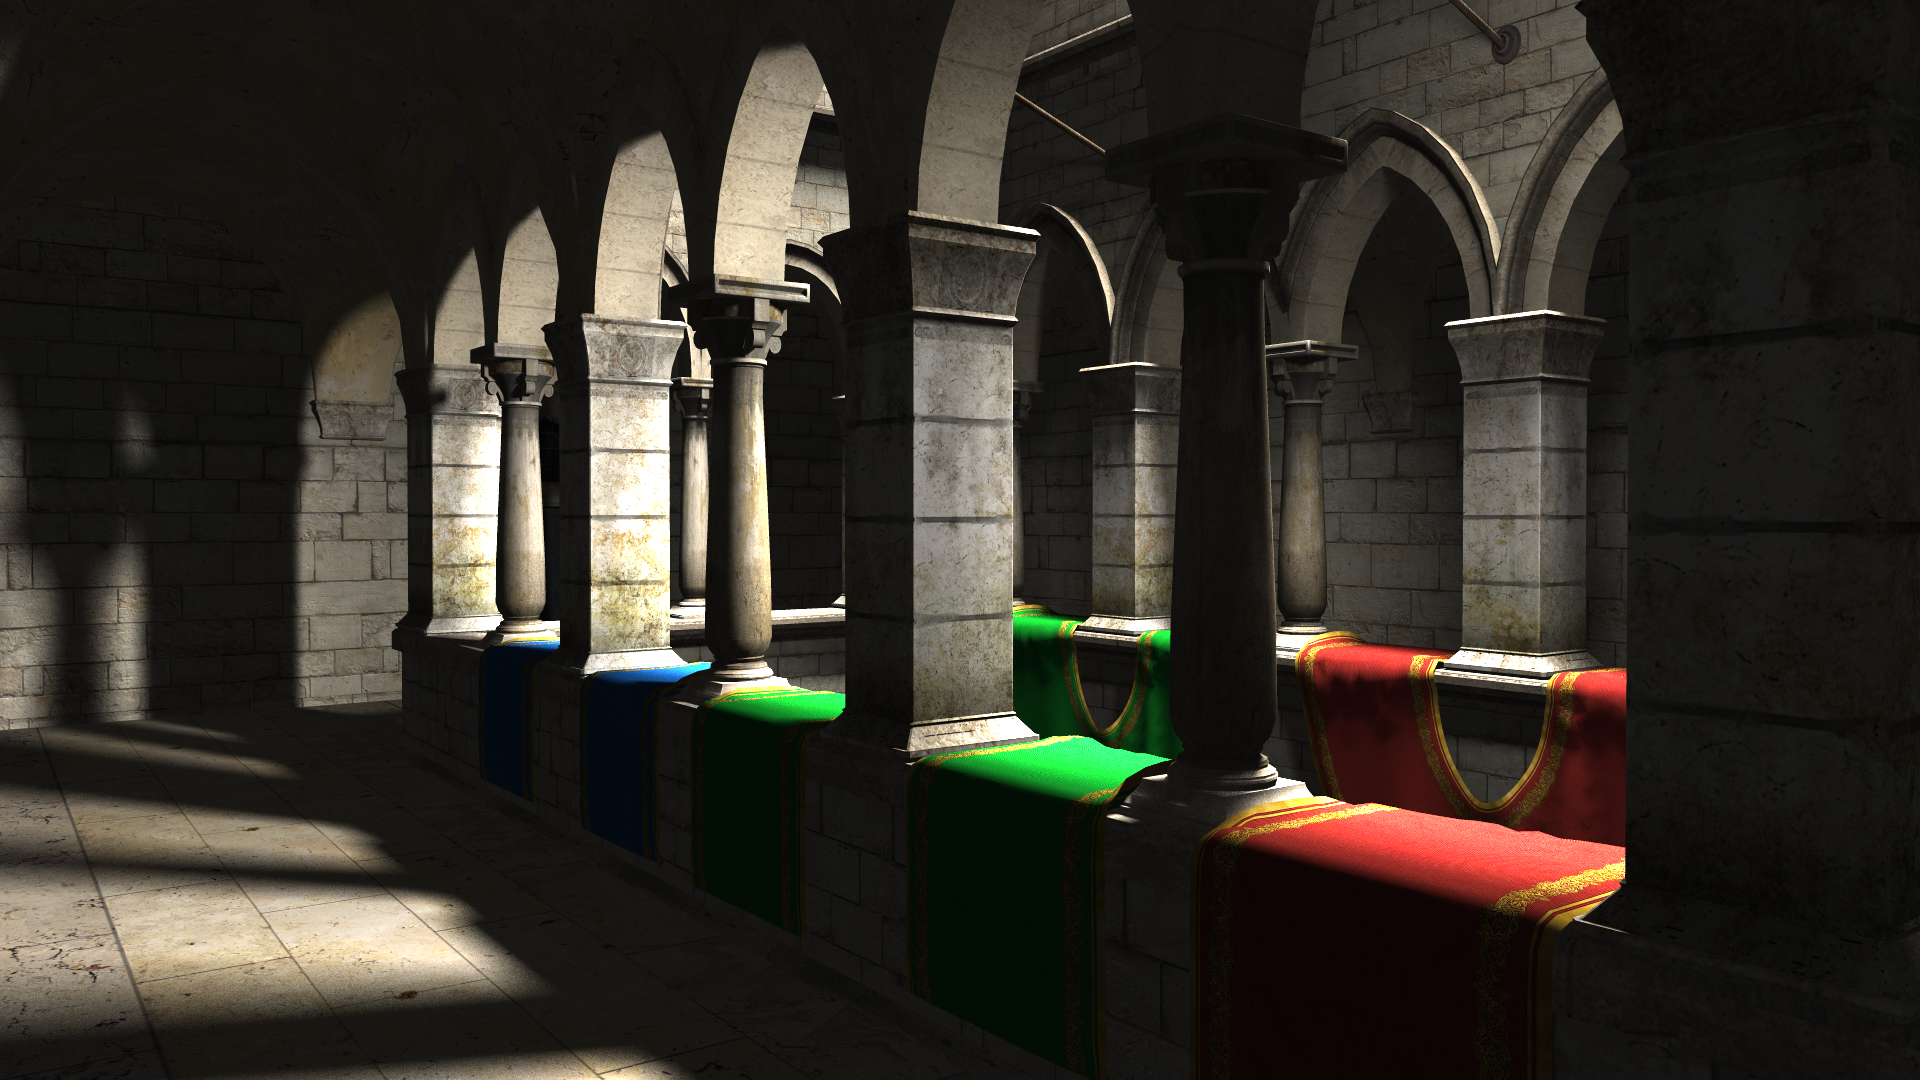
\includegraphics[width=\textwidth]{chapters/results/sponza_softshadows.png}
  \end{center}
  \caption{Test scene illuminated by 3 area lights, with 64 shadow samples per light. Rendering time was about 7 minutes.}
\end{figure}

\begin{figure}[htb]
  \begin{center}
    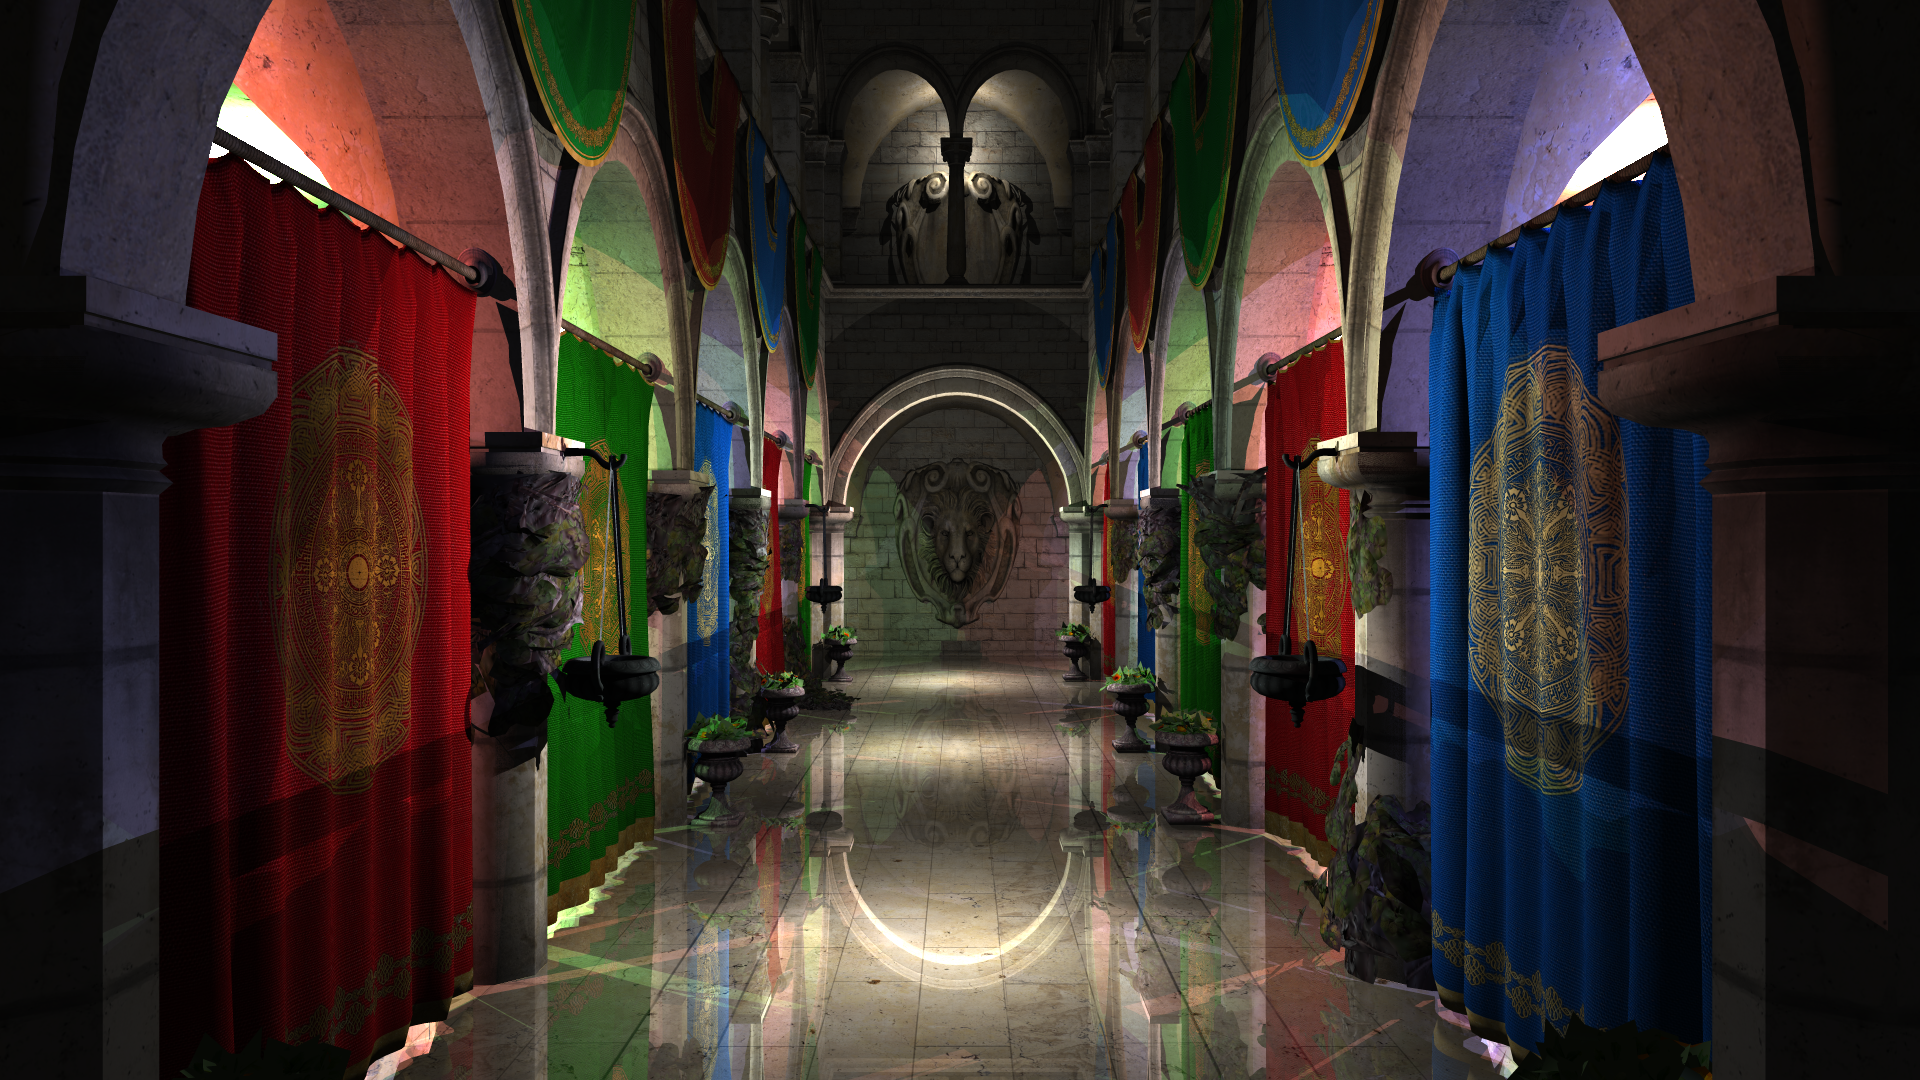
\includegraphics[width=\textwidth]{chapters/results/sponza_manypoint.png}
  \end{center}
  \caption{Test scene illuminated by 14 point lights. Rendering time was about 2.5 minutes.}
\end{figure}

\begin{figure}[htb]
  \begin{center}
    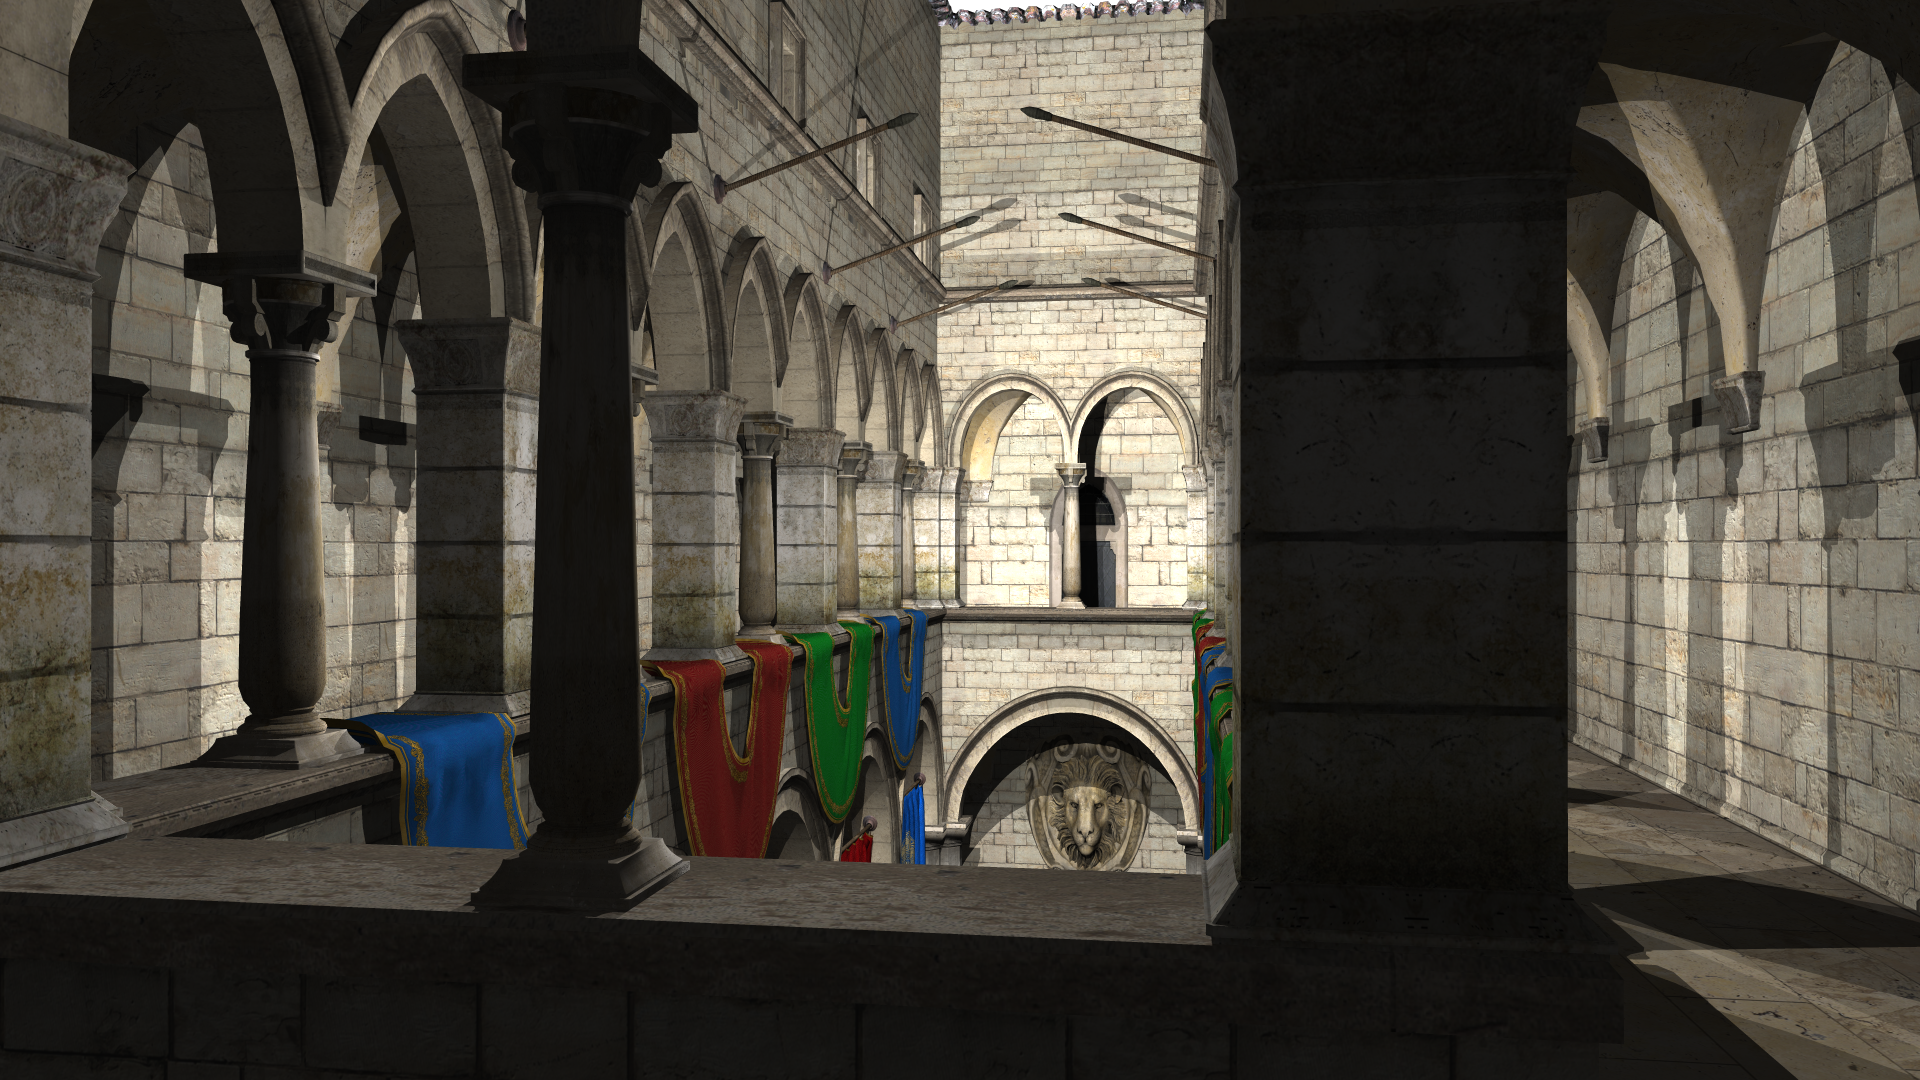
\includegraphics[width=\textwidth]{chapters/results/sponza_point.png}
  \end{center}
  \caption{Test scene illuminated by 3 point lights with no distance falloff. Rendering time was about 18 seconds.}
\end{figure}


\backmatter
\printbibliography

\end{document}